% LeadGuard paper, IEEE Journal of Biomedical and Health Informatics format (IEEEtran journal, two columns).
% Compile with pdflatex (twice) + bibtex. Every number comes from generated/numbers.tex and generated/tab_*.tex,
% written by make_numbers.py from results/*.csv, or from facts.tex (each line with its source).
\documentclass[journal]{IEEEtran}

\usepackage[utf8]{inputenc}
\usepackage[T1]{fontenc}
\usepackage{amsmath,amssymb}
\usepackage{graphicx}
\usepackage{booktabs}
\usepackage{adjustbox}
\usepackage{xcolor}
\usepackage{cite}
\usepackage{microtype}
\usepackage{tikz}
\usetikzlibrary{positioning,arrows.meta,fit,backgrounds,calc}
\usepackage[hidelinks]{hyperref}

\graphicspath{{figures/}}
% generated by paper/make_numbers.py from results/*.csv -- do not edit by hand
% each line: macro, value, source
\newcommand{\nTestRecords}{2{,}158} % sqa_agreement.csv: n_leads(clean)/12, test fold
\newcommand{\sqaGate}{0.984} % sqa_agreement.csv: min agreement_excl_band
\newcommand{\sqaGateType}{clip} % sqa_agreement.csv
\newcommand{\sqaMeanQClean}{0.997} % sqa_agreement.csv
\newcommand{\sqaEmgTestCorrupted}{0.514} % sqa_agreement.csv: emg_10db_test agreement_corrupted_leads
\newcommand{\sqaEmgTestBand}{0.250} % sqa_agreement.csv
\newcommand{\gpuMinutes}{25} % timing.csv: sum of seconds / 60
\newcommand{\secLgEdlRun}{200} % timing.csv: mean seconds per lg_edl run (first invocation)
\newcommand{\secResDropRun}{37} % timing.csv: mean seconds per resnet c1 run
\newcommand{\timeRatioLgRes}{5.4} % timing.csv: lg_edl / resnet c1 seconds per run
\newcommand{\aucLgEdlClean}{0.903} % table1.csv macro_auroc_mean
\newcommand{\aucLgEdlCleanPM}{0.903\,$\pm$\,0.001} % table1.csv
\newcommand{\foneLgEdlClean}{0.715} % table1.csv macro_f1_mean
\newcommand{\eceLgEdlClean}{0.032} % table1.csv ece_mean
\newcommand{\eceLgEdlCleanPM}{0.032\,$\pm$\,0.011} % table1.csv
\newcommand{\aucLgSoftClean}{0.906} % table1.csv macro_auroc_mean
\newcommand{\aucLgSoftCleanPM}{0.906} % table1.csv
\newcommand{\foneLgSoftClean}{0.715} % table1.csv macro_f1_mean
\newcommand{\eceLgSoftClean}{0.014} % table1.csv ece_mean
\newcommand{\eceLgSoftCleanPM}{0.014} % table1.csv
\newcommand{\aucLgHardClean}{0.907} % table1.csv macro_auroc_mean
\newcommand{\aucLgHardCleanPM}{0.907} % table1.csv
\newcommand{\foneLgHardClean}{0.726} % table1.csv macro_f1_mean
\newcommand{\eceLgHardClean}{0.012} % table1.csv ece_mean
\newcommand{\eceLgHardCleanPM}{0.012} % table1.csv
\newcommand{\aucResAttnClean}{0.909} % table1.csv macro_auroc_mean
\newcommand{\aucResAttnCleanPM}{0.909} % table1.csv
\newcommand{\foneResAttnClean}{0.726} % table1.csv macro_f1_mean
\newcommand{\eceResAttnClean}{0.014} % table1.csv ece_mean
\newcommand{\eceResAttnCleanPM}{0.014} % table1.csv
\newcommand{\aucResDropClean}{0.903} % table1.csv macro_auroc_mean
\newcommand{\aucResDropCleanPM}{0.903\,$\pm$\,0.000} % table1.csv
\newcommand{\foneResDropClean}{0.706} % table1.csv macro_f1_mean
\newcommand{\eceResDropClean}{0.015} % table1.csv ece_mean
\newcommand{\eceResDropCleanPM}{0.015\,$\pm$\,0.003} % table1.csv
\newcommand{\aucResCleanClean}{0.896} % table1.csv macro_auroc_mean
\newcommand{\aucResCleanCleanPM}{0.896} % table1.csv
\newcommand{\foneResCleanClean}{0.693} % table1.csv macro_f1_mean
\newcommand{\eceResCleanClean}{0.011} % table1.csv ece_mean
\newcommand{\eceResCleanCleanPM}{0.011} % table1.csv
\newcommand{\aucTransClean}{0.885} % table1.csv macro_auroc_mean
\newcommand{\aucTransCleanPM}{0.885} % table1.csv
\newcommand{\foneTransClean}{0.680} % table1.csv macro_f1_mean
\newcommand{\eceTransClean}{0.015} % table1.csv ece_mean
\newcommand{\eceTransCleanPM}{0.015} % table1.csv
\newcommand{\aucMlpClean}{0.722} % table1.csv macro_auroc_mean
\newcommand{\aucMlpCleanPM}{0.722} % table1.csv
\newcommand{\foneMlpClean}{0.486} % table1.csv macro_f1_mean
\newcommand{\eceMlpClean}{0.054} % table1.csv ece_mean
\newcommand{\eceMlpCleanPM}{0.054} % table1.csv
\newcommand{\aucXgbClean}{0.823} % table1.csv macro_auroc_mean
\newcommand{\aucXgbCleanPM}{0.823} % table1.csv
\newcommand{\foneXgbClean}{0.598} % table1.csv macro_f1_mean
\newcommand{\eceXgbClean}{0.013} % table1.csv ece_mean
\newcommand{\eceXgbCleanPM}{0.013} % table1.csv
\newcommand{\aucLgEdlKZero}{0.903} % random_loss.csv, mean over draws then seeds
\newcommand{\aucLgEdlKZeroPM}{0.903\,$\pm$\,0.001} % random_loss.csv
\newcommand{\aucLgEdlKTwo}{0.898} % random_loss.csv, mean over draws then seeds
\newcommand{\aucLgEdlKTwoPM}{0.898\,$\pm$\,0.001} % random_loss.csv
\newcommand{\aucLgEdlKFour}{0.891} % random_loss.csv, mean over draws then seeds
\newcommand{\aucLgEdlKFourPM}{0.891\,$\pm$\,0.001} % random_loss.csv
\newcommand{\aucLgEdlKSix}{0.878} % random_loss.csv, mean over draws then seeds
\newcommand{\aucLgEdlKSixPM}{0.878\,$\pm$\,0.000} % random_loss.csv
\newcommand{\aucLgEdlKEight}{0.857} % random_loss.csv, mean over draws then seeds
\newcommand{\aucLgEdlKEightPM}{0.857\,$\pm$\,0.001} % random_loss.csv
\newcommand{\aucLgEdlKTen}{0.804} % random_loss.csv, mean over draws then seeds
\newcommand{\aucLgEdlKTenPM}{0.804\,$\pm$\,0.002} % random_loss.csv
\newcommand{\aucLgSoftKZero}{0.906} % random_loss.csv, mean over draws then seeds
\newcommand{\aucLgSoftKZeroPM}{0.906} % random_loss.csv
\newcommand{\aucLgSoftKTwo}{0.902} % random_loss.csv, mean over draws then seeds
\newcommand{\aucLgSoftKTwoPM}{0.902} % random_loss.csv
\newcommand{\aucLgSoftKFour}{0.897} % random_loss.csv, mean over draws then seeds
\newcommand{\aucLgSoftKFourPM}{0.897} % random_loss.csv
\newcommand{\aucLgSoftKSix}{0.883} % random_loss.csv, mean over draws then seeds
\newcommand{\aucLgSoftKSixPM}{0.883} % random_loss.csv
\newcommand{\aucLgSoftKEight}{0.863} % random_loss.csv, mean over draws then seeds
\newcommand{\aucLgSoftKEightPM}{0.863} % random_loss.csv
\newcommand{\aucLgSoftKTen}{0.811} % random_loss.csv, mean over draws then seeds
\newcommand{\aucLgSoftKTenPM}{0.811} % random_loss.csv
\newcommand{\aucLgHardKZero}{0.907} % random_loss.csv, mean over draws then seeds
\newcommand{\aucLgHardKZeroPM}{0.907} % random_loss.csv
\newcommand{\aucLgHardKTwo}{0.903} % random_loss.csv, mean over draws then seeds
\newcommand{\aucLgHardKTwoPM}{0.903} % random_loss.csv
\newcommand{\aucLgHardKFour}{0.898} % random_loss.csv, mean over draws then seeds
\newcommand{\aucLgHardKFourPM}{0.898} % random_loss.csv
\newcommand{\aucLgHardKSix}{0.884} % random_loss.csv, mean over draws then seeds
\newcommand{\aucLgHardKSixPM}{0.884} % random_loss.csv
\newcommand{\aucLgHardKEight}{0.865} % random_loss.csv, mean over draws then seeds
\newcommand{\aucLgHardKEightPM}{0.865} % random_loss.csv
\newcommand{\aucLgHardKTen}{0.812} % random_loss.csv, mean over draws then seeds
\newcommand{\aucLgHardKTenPM}{0.812} % random_loss.csv
\newcommand{\aucResAttnKZero}{0.909} % random_loss.csv, mean over draws then seeds
\newcommand{\aucResAttnKZeroPM}{0.909} % random_loss.csv
\newcommand{\aucResAttnKTwo}{0.903} % random_loss.csv, mean over draws then seeds
\newcommand{\aucResAttnKTwoPM}{0.903} % random_loss.csv
\newcommand{\aucResAttnKFour}{0.897} % random_loss.csv, mean over draws then seeds
\newcommand{\aucResAttnKFourPM}{0.897} % random_loss.csv
\newcommand{\aucResAttnKSix}{0.882} % random_loss.csv, mean over draws then seeds
\newcommand{\aucResAttnKSixPM}{0.882} % random_loss.csv
\newcommand{\aucResAttnKEight}{0.861} % random_loss.csv, mean over draws then seeds
\newcommand{\aucResAttnKEightPM}{0.861} % random_loss.csv
\newcommand{\aucResAttnKTen}{0.810} % random_loss.csv, mean over draws then seeds
\newcommand{\aucResAttnKTenPM}{0.810} % random_loss.csv
\newcommand{\aucResDropKZero}{0.903} % random_loss.csv, mean over draws then seeds
\newcommand{\aucResDropKZeroPM}{0.903\,$\pm$\,0.000} % random_loss.csv
\newcommand{\aucResDropKTwo}{0.897} % random_loss.csv, mean over draws then seeds
\newcommand{\aucResDropKTwoPM}{0.897\,$\pm$\,0.001} % random_loss.csv
\newcommand{\aucResDropKFour}{0.891} % random_loss.csv, mean over draws then seeds
\newcommand{\aucResDropKFourPM}{0.891\,$\pm$\,0.001} % random_loss.csv
\newcommand{\aucResDropKSix}{0.875} % random_loss.csv, mean over draws then seeds
\newcommand{\aucResDropKSixPM}{0.875\,$\pm$\,0.002} % random_loss.csv
\newcommand{\aucResDropKEight}{0.853} % random_loss.csv, mean over draws then seeds
\newcommand{\aucResDropKEightPM}{0.853\,$\pm$\,0.002} % random_loss.csv
\newcommand{\aucResDropKTen}{0.800} % random_loss.csv, mean over draws then seeds
\newcommand{\aucResDropKTenPM}{0.800\,$\pm$\,0.007} % random_loss.csv
\newcommand{\aucResCleanKZero}{0.896} % random_loss.csv, mean over draws then seeds
\newcommand{\aucResCleanKZeroPM}{0.896} % random_loss.csv
\newcommand{\aucResCleanKTwo}{0.872} % random_loss.csv, mean over draws then seeds
\newcommand{\aucResCleanKTwoPM}{0.872} % random_loss.csv
\newcommand{\aucResCleanKFour}{0.837} % random_loss.csv, mean over draws then seeds
\newcommand{\aucResCleanKFourPM}{0.837} % random_loss.csv
\newcommand{\aucResCleanKSix}{0.778} % random_loss.csv, mean over draws then seeds
\newcommand{\aucResCleanKSixPM}{0.778} % random_loss.csv
\newcommand{\aucResCleanKEight}{0.705} % random_loss.csv, mean over draws then seeds
\newcommand{\aucResCleanKEightPM}{0.705} % random_loss.csv
\newcommand{\aucResCleanKTen}{0.613} % random_loss.csv, mean over draws then seeds
\newcommand{\aucResCleanKTenPM}{0.613} % random_loss.csv
\newcommand{\aucTransKZero}{0.885} % random_loss.csv, mean over draws then seeds
\newcommand{\aucTransKZeroPM}{0.885} % random_loss.csv
\newcommand{\aucTransKTwo}{0.881} % random_loss.csv, mean over draws then seeds
\newcommand{\aucTransKTwoPM}{0.881} % random_loss.csv
\newcommand{\aucTransKFour}{0.874} % random_loss.csv, mean over draws then seeds
\newcommand{\aucTransKFourPM}{0.874} % random_loss.csv
\newcommand{\aucTransKSix}{0.856} % random_loss.csv, mean over draws then seeds
\newcommand{\aucTransKSixPM}{0.856} % random_loss.csv
\newcommand{\aucTransKEight}{0.827} % random_loss.csv, mean over draws then seeds
\newcommand{\aucTransKEightPM}{0.827} % random_loss.csv
\newcommand{\aucTransKTen}{0.756} % random_loss.csv, mean over draws then seeds
\newcommand{\aucTransKTenPM}{0.756} % random_loss.csv
\newcommand{\aucMlpKZero}{0.722} % random_loss.csv, mean over draws then seeds
\newcommand{\aucMlpKZeroPM}{0.722} % random_loss.csv
\newcommand{\aucMlpKTwo}{0.712} % random_loss.csv, mean over draws then seeds
\newcommand{\aucMlpKTwoPM}{0.712} % random_loss.csv
\newcommand{\aucMlpKFour}{0.700} % random_loss.csv, mean over draws then seeds
\newcommand{\aucMlpKFourPM}{0.700} % random_loss.csv
\newcommand{\aucMlpKSix}{0.682} % random_loss.csv, mean over draws then seeds
\newcommand{\aucMlpKSixPM}{0.682} % random_loss.csv
\newcommand{\aucMlpKEight}{0.654} % random_loss.csv, mean over draws then seeds
\newcommand{\aucMlpKEightPM}{0.654} % random_loss.csv
\newcommand{\aucMlpKTen}{0.604} % random_loss.csv, mean over draws then seeds
\newcommand{\aucMlpKTenPM}{0.604} % random_loss.csv
\newcommand{\aucXgbKZero}{0.823} % random_loss.csv, mean over draws then seeds
\newcommand{\aucXgbKZeroPM}{0.823} % random_loss.csv
\newcommand{\aucXgbKTwo}{0.752} % random_loss.csv, mean over draws then seeds
\newcommand{\aucXgbKTwoPM}{0.752} % random_loss.csv
\newcommand{\aucXgbKFour}{0.700} % random_loss.csv, mean over draws then seeds
\newcommand{\aucXgbKFourPM}{0.700} % random_loss.csv
\newcommand{\aucXgbKSix}{0.655} % random_loss.csv, mean over draws then seeds
\newcommand{\aucXgbKSixPM}{0.655} % random_loss.csv
\newcommand{\aucXgbKEight}{0.617} % random_loss.csv, mean over draws then seeds
\newcommand{\aucXgbKEightPM}{0.617} % random_loss.csv
\newcommand{\aucXgbKTen}{0.581} % random_loss.csv, mean over draws then seeds
\newcommand{\aucXgbKTenPM}{0.581} % random_loss.csv
\newcommand{\gainDropKTen}{0.187} % random_loss.csv: resnet_c1 - resnet_c0 at k=10
\newcommand{\lossResCleanKTen}{0.283} % random_loss.csv
\newcommand{\lossResDropKTen}{0.103} % random_loss.csv
\newcommand{\lossLgEdlKTen}{0.099} % random_loss.csv
\newcommand{\gapAttnResKTen}{0.012} % random_loss.csv: best attention variant minus resnet_c1 at k=10
\newcommand{\seedStdLgEdlMaxLoss}{0.002} % random_loss.csv: largest LG-EDL seed std over k=2..10
\newcommand{\foneLgEdlKZero}{0.715} % random_loss.csv macro_f1, mean over draws then seeds
\newcommand{\foneLgEdlKTwo}{0.708} % random_loss.csv macro_f1, mean over draws then seeds
\newcommand{\foneLgEdlKFour}{0.698} % random_loss.csv macro_f1, mean over draws then seeds
\newcommand{\foneLgEdlKSix}{0.674} % random_loss.csv macro_f1, mean over draws then seeds
\newcommand{\foneLgEdlKEight}{0.642} % random_loss.csv macro_f1, mean over draws then seeds
\newcommand{\foneLgEdlKTen}{0.554} % random_loss.csv macro_f1, mean over draws then seeds
\newcommand{\foneLgSoftKZero}{0.715} % random_loss.csv macro_f1, mean over draws then seeds
\newcommand{\foneLgSoftKTwo}{0.710} % random_loss.csv macro_f1, mean over draws then seeds
\newcommand{\foneLgSoftKFour}{0.704} % random_loss.csv macro_f1, mean over draws then seeds
\newcommand{\foneLgSoftKSix}{0.681} % random_loss.csv macro_f1, mean over draws then seeds
\newcommand{\foneLgSoftKEight}{0.645} % random_loss.csv macro_f1, mean over draws then seeds
\newcommand{\foneLgSoftKTen}{0.566} % random_loss.csv macro_f1, mean over draws then seeds
\newcommand{\foneLgHardKZero}{0.726} % random_loss.csv macro_f1, mean over draws then seeds
\newcommand{\foneLgHardKTwo}{0.715} % random_loss.csv macro_f1, mean over draws then seeds
\newcommand{\foneLgHardKFour}{0.708} % random_loss.csv macro_f1, mean over draws then seeds
\newcommand{\foneLgHardKSix}{0.685} % random_loss.csv macro_f1, mean over draws then seeds
\newcommand{\foneLgHardKEight}{0.652} % random_loss.csv macro_f1, mean over draws then seeds
\newcommand{\foneLgHardKTen}{0.570} % random_loss.csv macro_f1, mean over draws then seeds
\newcommand{\foneResAttnKZero}{0.726} % random_loss.csv macro_f1, mean over draws then seeds
\newcommand{\foneResAttnKTwo}{0.716} % random_loss.csv macro_f1, mean over draws then seeds
\newcommand{\foneResAttnKFour}{0.711} % random_loss.csv macro_f1, mean over draws then seeds
\newcommand{\foneResAttnKSix}{0.679} % random_loss.csv macro_f1, mean over draws then seeds
\newcommand{\foneResAttnKEight}{0.647} % random_loss.csv macro_f1, mean over draws then seeds
\newcommand{\foneResAttnKTen}{0.570} % random_loss.csv macro_f1, mean over draws then seeds
\newcommand{\foneResDropKZero}{0.706} % random_loss.csv macro_f1, mean over draws then seeds
\newcommand{\foneResDropKTwo}{0.696} % random_loss.csv macro_f1, mean over draws then seeds
\newcommand{\foneResDropKFour}{0.688} % random_loss.csv macro_f1, mean over draws then seeds
\newcommand{\foneResDropKSix}{0.663} % random_loss.csv macro_f1, mean over draws then seeds
\newcommand{\foneResDropKEight}{0.628} % random_loss.csv macro_f1, mean over draws then seeds
\newcommand{\foneResDropKTen}{0.548} % random_loss.csv macro_f1, mean over draws then seeds
\newcommand{\foneResCleanKZero}{0.693} % random_loss.csv macro_f1, mean over draws then seeds
\newcommand{\foneResCleanKTwo}{0.648} % random_loss.csv macro_f1, mean over draws then seeds
\newcommand{\foneResCleanKFour}{0.574} % random_loss.csv macro_f1, mean over draws then seeds
\newcommand{\foneResCleanKSix}{0.458} % random_loss.csv macro_f1, mean over draws then seeds
\newcommand{\foneResCleanKEight}{0.345} % random_loss.csv macro_f1, mean over draws then seeds
\newcommand{\foneResCleanKTen}{0.259} % random_loss.csv macro_f1, mean over draws then seeds
\newcommand{\foneTransKZero}{0.680} % random_loss.csv macro_f1, mean over draws then seeds
\newcommand{\foneTransKTwo}{0.676} % random_loss.csv macro_f1, mean over draws then seeds
\newcommand{\foneTransKFour}{0.668} % random_loss.csv macro_f1, mean over draws then seeds
\newcommand{\foneTransKSix}{0.638} % random_loss.csv macro_f1, mean over draws then seeds
\newcommand{\foneTransKEight}{0.598} % random_loss.csv macro_f1, mean over draws then seeds
\newcommand{\foneTransKTen}{0.503} % random_loss.csv macro_f1, mean over draws then seeds
\newcommand{\foneMlpKZero}{0.486} % random_loss.csv macro_f1, mean over draws then seeds
\newcommand{\foneMlpKTwo}{0.477} % random_loss.csv macro_f1, mean over draws then seeds
\newcommand{\foneMlpKFour}{0.465} % random_loss.csv macro_f1, mean over draws then seeds
\newcommand{\foneMlpKSix}{0.447} % random_loss.csv macro_f1, mean over draws then seeds
\newcommand{\foneMlpKEight}{0.426} % random_loss.csv macro_f1, mean over draws then seeds
\newcommand{\foneMlpKTen}{0.406} % random_loss.csv macro_f1, mean over draws then seeds
\newcommand{\foneXgbKZero}{0.598} % random_loss.csv macro_f1, mean over draws then seeds
\newcommand{\foneXgbKTwo}{0.482} % random_loss.csv macro_f1, mean over draws then seeds
\newcommand{\foneXgbKFour}{0.388} % random_loss.csv macro_f1, mean over draws then seeds
\newcommand{\foneXgbKSix}{0.325} % random_loss.csv macro_f1, mean over draws then seeds
\newcommand{\foneXgbKEight}{0.295} % random_loss.csv macro_f1, mean over draws then seeds
\newcommand{\foneXgbKTen}{0.280} % random_loss.csv macro_f1, mean over draws then seeds
\newcommand{\eceLgEdlKZero}{0.032} % random_loss.csv ece, mean over draws then seeds
\newcommand{\eceLgEdlKTwo}{0.030} % random_loss.csv ece, mean over draws then seeds
\newcommand{\eceLgEdlKFour}{0.025} % random_loss.csv ece, mean over draws then seeds
\newcommand{\eceLgEdlKSix}{0.020} % random_loss.csv ece, mean over draws then seeds
\newcommand{\eceLgEdlKEight}{0.020} % random_loss.csv ece, mean over draws then seeds
\newcommand{\eceLgEdlKTen}{0.056} % random_loss.csv ece, mean over draws then seeds
\newcommand{\eceLgSoftKZero}{0.014} % random_loss.csv ece, mean over draws then seeds
\newcommand{\eceLgSoftKTwo}{0.014} % random_loss.csv ece, mean over draws then seeds
\newcommand{\eceLgSoftKFour}{0.017} % random_loss.csv ece, mean over draws then seeds
\newcommand{\eceLgSoftKSix}{0.022} % random_loss.csv ece, mean over draws then seeds
\newcommand{\eceLgSoftKEight}{0.033} % random_loss.csv ece, mean over draws then seeds
\newcommand{\eceLgSoftKTen}{0.063} % random_loss.csv ece, mean over draws then seeds
\newcommand{\eceLgHardKZero}{0.012} % random_loss.csv ece, mean over draws then seeds
\newcommand{\eceLgHardKTwo}{0.012} % random_loss.csv ece, mean over draws then seeds
\newcommand{\eceLgHardKFour}{0.013} % random_loss.csv ece, mean over draws then seeds
\newcommand{\eceLgHardKSix}{0.021} % random_loss.csv ece, mean over draws then seeds
\newcommand{\eceLgHardKEight}{0.030} % random_loss.csv ece, mean over draws then seeds
\newcommand{\eceLgHardKTen}{0.059} % random_loss.csv ece, mean over draws then seeds
\newcommand{\eceResAttnKZero}{0.014} % random_loss.csv ece, mean over draws then seeds
\newcommand{\eceResAttnKTwo}{0.012} % random_loss.csv ece, mean over draws then seeds
\newcommand{\eceResAttnKFour}{0.013} % random_loss.csv ece, mean over draws then seeds
\newcommand{\eceResAttnKSix}{0.015} % random_loss.csv ece, mean over draws then seeds
\newcommand{\eceResAttnKEight}{0.017} % random_loss.csv ece, mean over draws then seeds
\newcommand{\eceResAttnKTen}{0.023} % random_loss.csv ece, mean over draws then seeds
\newcommand{\eceResDropKZero}{0.015} % random_loss.csv ece, mean over draws then seeds
\newcommand{\eceResDropKTwo}{0.014} % random_loss.csv ece, mean over draws then seeds
\newcommand{\eceResDropKFour}{0.016} % random_loss.csv ece, mean over draws then seeds
\newcommand{\eceResDropKSix}{0.017} % random_loss.csv ece, mean over draws then seeds
\newcommand{\eceResDropKEight}{0.020} % random_loss.csv ece, mean over draws then seeds
\newcommand{\eceResDropKTen}{0.031} % random_loss.csv ece, mean over draws then seeds
\newcommand{\eceResCleanKZero}{0.011} % random_loss.csv ece, mean over draws then seeds
\newcommand{\eceResCleanKTwo}{0.021} % random_loss.csv ece, mean over draws then seeds
\newcommand{\eceResCleanKFour}{0.056} % random_loss.csv ece, mean over draws then seeds
\newcommand{\eceResCleanKSix}{0.135} % random_loss.csv ece, mean over draws then seeds
\newcommand{\eceResCleanKEight}{0.226} % random_loss.csv ece, mean over draws then seeds
\newcommand{\eceResCleanKTen}{0.301} % random_loss.csv ece, mean over draws then seeds
\newcommand{\eceTransKZero}{0.015} % random_loss.csv ece, mean over draws then seeds
\newcommand{\eceTransKTwo}{0.017} % random_loss.csv ece, mean over draws then seeds
\newcommand{\eceTransKFour}{0.016} % random_loss.csv ece, mean over draws then seeds
\newcommand{\eceTransKSix}{0.017} % random_loss.csv ece, mean over draws then seeds
\newcommand{\eceTransKEight}{0.019} % random_loss.csv ece, mean over draws then seeds
\newcommand{\eceTransKTen}{0.034} % random_loss.csv ece, mean over draws then seeds
\newcommand{\eceMlpKZero}{0.054} % random_loss.csv ece, mean over draws then seeds
\newcommand{\eceMlpKTwo}{0.068} % random_loss.csv ece, mean over draws then seeds
\newcommand{\eceMlpKFour}{0.088} % random_loss.csv ece, mean over draws then seeds
\newcommand{\eceMlpKSix}{0.110} % random_loss.csv ece, mean over draws then seeds
\newcommand{\eceMlpKEight}{0.137} % random_loss.csv ece, mean over draws then seeds
\newcommand{\eceMlpKTen}{0.168} % random_loss.csv ece, mean over draws then seeds
\newcommand{\eceXgbKZero}{0.013} % random_loss.csv ece, mean over draws then seeds
\newcommand{\eceXgbKTwo}{0.038} % random_loss.csv ece, mean over draws then seeds
\newcommand{\eceXgbKFour}{0.108} % random_loss.csv ece, mean over draws then seeds
\newcommand{\eceXgbKSix}{0.183} % random_loss.csv ece, mean over draws then seeds
\newcommand{\eceXgbKEight}{0.250} % random_loss.csv ece, mean over draws then seeds
\newcommand{\eceXgbKTen}{0.298} % random_loss.csv ece, mean over draws then seeds
\newcommand{\aucLgEdlPrec}{0.871} % group_loss.csv
\newcommand{\aucLgEdlLimb}{0.869} % group_loss.csv
\newcommand{\aucLgEdlVOneThree}{0.882} % group_loss.csv
\newcommand{\aucLgSoftPrec}{0.877} % group_loss.csv
\newcommand{\aucLgSoftLimb}{0.870} % group_loss.csv
\newcommand{\aucLgSoftVOneThree}{0.887} % group_loss.csv
\newcommand{\aucLgHardPrec}{0.878} % group_loss.csv
\newcommand{\aucLgHardLimb}{0.869} % group_loss.csv
\newcommand{\aucLgHardVOneThree}{0.888} % group_loss.csv
\newcommand{\aucResAttnPrec}{0.876} % group_loss.csv
\newcommand{\aucResAttnLimb}{0.874} % group_loss.csv
\newcommand{\aucResAttnVOneThree}{0.888} % group_loss.csv
\newcommand{\aucResDropPrec}{0.873} % group_loss.csv
\newcommand{\aucResDropLimb}{0.868} % group_loss.csv
\newcommand{\aucResDropVOneThree}{0.882} % group_loss.csv
\newcommand{\aucResCleanPrec}{0.747} % group_loss.csv
\newcommand{\aucResCleanLimb}{0.809} % group_loss.csv
\newcommand{\aucResCleanVOneThree}{0.851} % group_loss.csv
\newcommand{\aucTransPrec}{0.853} % group_loss.csv
\newcommand{\aucTransLimb}{0.845} % group_loss.csv
\newcommand{\aucTransVOneThree}{0.864} % group_loss.csv
\newcommand{\aucMlpPrec}{0.661} % group_loss.csv
\newcommand{\aucMlpLimb}{0.679} % group_loss.csv
\newcommand{\aucMlpVOneThree}{0.669} % group_loss.csv
\newcommand{\aucXgbPrec}{0.666} % group_loss.csv
\newcommand{\aucXgbLimb}{0.734} % group_loss.csv
\newcommand{\aucXgbVOneThree}{0.743} % group_loss.csv
\newcommand{\aucLgEdlEmgTwo}{0.901} % artifact.csv
\newcommand{\aucLgEdlEmgFour}{0.900} % artifact.csv
\newcommand{\aucLgEdlEmgSix}{0.898} % artifact.csv
\newcommand{\aucLgEdlWanderTwo}{0.898} % artifact.csv
\newcommand{\aucLgEdlWanderFour}{0.896} % artifact.csv
\newcommand{\aucLgEdlWanderSix}{0.891} % artifact.csv
\newcommand{\aucLgEdlClipTwo}{0.901} % artifact.csv
\newcommand{\aucLgEdlClipFour}{0.894} % artifact.csv
\newcommand{\aucLgEdlClipSix}{0.889} % artifact.csv
\newcommand{\aucLgSoftEmgTwo}{0.904} % artifact.csv
\newcommand{\aucLgSoftEmgFour}{0.903} % artifact.csv
\newcommand{\aucLgSoftEmgSix}{0.900} % artifact.csv
\newcommand{\aucLgSoftWanderTwo}{0.901} % artifact.csv
\newcommand{\aucLgSoftWanderFour}{0.899} % artifact.csv
\newcommand{\aucLgSoftWanderSix}{0.895} % artifact.csv
\newcommand{\aucLgSoftClipTwo}{0.905} % artifact.csv
\newcommand{\aucLgSoftClipFour}{0.898} % artifact.csv
\newcommand{\aucLgSoftClipSix}{0.893} % artifact.csv
\newcommand{\aucLgHardEmgTwo}{0.904} % artifact.csv
\newcommand{\aucLgHardEmgFour}{0.899} % artifact.csv
\newcommand{\aucLgHardEmgSix}{0.895} % artifact.csv
\newcommand{\aucLgHardWanderTwo}{0.903} % artifact.csv
\newcommand{\aucLgHardWanderFour}{0.899} % artifact.csv
\newcommand{\aucLgHardWanderSix}{0.894} % artifact.csv
\newcommand{\aucLgHardClipTwo}{0.905} % artifact.csv
\newcommand{\aucLgHardClipFour}{0.898} % artifact.csv
\newcommand{\aucLgHardClipSix}{0.890} % artifact.csv
\newcommand{\aucResAttnEmgTwo}{0.907} % artifact.csv
\newcommand{\aucResAttnEmgFour}{0.906} % artifact.csv
\newcommand{\aucResAttnEmgSix}{0.904} % artifact.csv
\newcommand{\aucResAttnWanderTwo}{0.905} % artifact.csv
\newcommand{\aucResAttnWanderFour}{0.904} % artifact.csv
\newcommand{\aucResAttnWanderSix}{0.903} % artifact.csv
\newcommand{\aucResAttnClipTwo}{0.907} % artifact.csv
\newcommand{\aucResAttnClipFour}{0.899} % artifact.csv
\newcommand{\aucResAttnClipSix}{0.893} % artifact.csv
\newcommand{\aucResDropEmgTwo}{0.903} % artifact.csv
\newcommand{\aucResDropEmgFour}{0.903} % artifact.csv
\newcommand{\aucResDropEmgSix}{0.903} % artifact.csv
\newcommand{\aucResDropWanderTwo}{0.904} % artifact.csv
\newcommand{\aucResDropWanderFour}{0.901} % artifact.csv
\newcommand{\aucResDropWanderSix}{0.899} % artifact.csv
\newcommand{\aucResDropClipTwo}{0.902} % artifact.csv
\newcommand{\aucResDropClipFour}{0.896} % artifact.csv
\newcommand{\aucResDropClipSix}{0.894} % artifact.csv
\newcommand{\aucResCleanEmgTwo}{0.895} % artifact.csv
\newcommand{\aucResCleanEmgFour}{0.895} % artifact.csv
\newcommand{\aucResCleanEmgSix}{0.896} % artifact.csv
\newcommand{\aucResCleanWanderTwo}{0.880} % artifact.csv
\newcommand{\aucResCleanWanderFour}{0.868} % artifact.csv
\newcommand{\aucResCleanWanderSix}{0.844} % artifact.csv
\newcommand{\aucResCleanClipTwo}{0.892} % artifact.csv
\newcommand{\aucResCleanClipFour}{0.883} % artifact.csv
\newcommand{\aucResCleanClipSix}{0.877} % artifact.csv
\newcommand{\aucTransEmgTwo}{0.885} % artifact.csv
\newcommand{\aucTransEmgFour}{0.885} % artifact.csv
\newcommand{\aucTransEmgSix}{0.885} % artifact.csv
\newcommand{\aucTransWanderTwo}{0.883} % artifact.csv
\newcommand{\aucTransWanderFour}{0.883} % artifact.csv
\newcommand{\aucTransWanderSix}{0.875} % artifact.csv
\newcommand{\aucTransClipTwo}{0.885} % artifact.csv
\newcommand{\aucTransClipFour}{0.881} % artifact.csv
\newcommand{\aucTransClipSix}{0.880} % artifact.csv
\newcommand{\aucMlpEmgTwo}{0.722} % artifact.csv
\newcommand{\aucMlpEmgFour}{0.721} % artifact.csv
\newcommand{\aucMlpEmgSix}{0.721} % artifact.csv
\newcommand{\aucMlpWanderTwo}{0.710} % artifact.csv
\newcommand{\aucMlpWanderFour}{0.702} % artifact.csv
\newcommand{\aucMlpWanderSix}{0.684} % artifact.csv
\newcommand{\aucMlpClipTwo}{0.724} % artifact.csv
\newcommand{\aucMlpClipFour}{0.719} % artifact.csv
\newcommand{\aucMlpClipSix}{0.723} % artifact.csv
\newcommand{\aucXgbEmgTwo}{0.821} % artifact.csv
\newcommand{\aucXgbEmgFour}{0.817} % artifact.csv
\newcommand{\aucXgbEmgSix}{0.814} % artifact.csv
\newcommand{\aucXgbWanderTwo}{0.801} % artifact.csv
\newcommand{\aucXgbWanderFour}{0.780} % artifact.csv
\newcommand{\aucXgbWanderSix}{0.749} % artifact.csv
\newcommand{\aucXgbClipTwo}{0.790} % artifact.csv
\newcommand{\aucXgbClipFour}{0.750} % artifact.csv
\newcommand{\aucXgbClipSix}{0.727} % artifact.csv
\newcommand{\bootNRows}{28} % bootstrap_ci.csv rows excluding random_0 (= clean)
\newcommand{\bootNSig}{4} % bootstrap_ci.csv: CI excludes 0
\newcommand{\bootNSigNeg}{4} % bootstrap_ci.csv: CI entirely below 0
\newcommand{\bootNSigPos}{0} % bootstrap_ci.csv: CI entirely above 0
\newcommand{\bootNBoot}{1000} % bootstrap_ci.csv n_boot
\newcommand{\bootCleanDiff}{$-$0.0006} % bootstrap_ci.csv diff
\newcommand{\bootCleanCI}{[$-$0.0053, +0.0039]} % bootstrap_ci.csv ci_low/ci_high
\newcommand{\bootKTwoDADiff}{0.0000} % bootstrap_ci.csv diff
\newcommand{\bootKTwoDACI}{[$-$0.0052, +0.0051]} % bootstrap_ci.csv ci_low/ci_high
\newcommand{\bootKTwoDBDiff}{+0.0023} % bootstrap_ci.csv diff
\newcommand{\bootKTwoDBCI}{[$-$0.0027, +0.0071]} % bootstrap_ci.csv ci_low/ci_high
\newcommand{\bootKTwoDCDiff}{+0.0007} % bootstrap_ci.csv diff
\newcommand{\bootKTwoDCCI}{[$-$0.0044, +0.0056]} % bootstrap_ci.csv ci_low/ci_high
\newcommand{\bootKFourDADiff}{$-$0.0009} % bootstrap_ci.csv diff
\newcommand{\bootKFourDACI}{[$-$0.0062, +0.0044]} % bootstrap_ci.csv ci_low/ci_high
\newcommand{\bootKFourDBDiff}{+0.0021} % bootstrap_ci.csv diff
\newcommand{\bootKFourDBCI}{[$-$0.0036, +0.0073]} % bootstrap_ci.csv ci_low/ci_high
\newcommand{\bootKFourDCDiff}{0.0000} % bootstrap_ci.csv diff
\newcommand{\bootKFourDCCI}{[$-$0.0058, +0.0053]} % bootstrap_ci.csv ci_low/ci_high
\newcommand{\bootKSixDADiff}{+0.0064} % bootstrap_ci.csv diff
\newcommand{\bootKSixDACI}{[0.0000, +0.0126]} % bootstrap_ci.csv ci_low/ci_high
\newcommand{\bootKSixDBDiff}{$-$0.0011} % bootstrap_ci.csv diff
\newcommand{\bootKSixDBCI}{[$-$0.0071, +0.0054]} % bootstrap_ci.csv ci_low/ci_high
\newcommand{\bootKSixDCDiff}{+0.0024} % bootstrap_ci.csv diff
\newcommand{\bootKSixDCCI}{[$-$0.0040, +0.0086]} % bootstrap_ci.csv ci_low/ci_high
\newcommand{\bootKEightDADiff}{+0.0036} % bootstrap_ci.csv diff
\newcommand{\bootKEightDACI}{[$-$0.0039, +0.0109]} % bootstrap_ci.csv ci_low/ci_high
\newcommand{\bootKEightDBDiff}{+0.0054} % bootstrap_ci.csv diff
\newcommand{\bootKEightDBCI}{[$-$0.0022, +0.0124]} % bootstrap_ci.csv ci_low/ci_high
\newcommand{\bootKEightDCDiff}{+0.0011} % bootstrap_ci.csv diff
\newcommand{\bootKEightDCCI}{[$-$0.0054, +0.0086]} % bootstrap_ci.csv ci_low/ci_high
\newcommand{\bootKTenDADiff}{+0.0044} % bootstrap_ci.csv diff
\newcommand{\bootKTenDACI}{[$-$0.0043, +0.0137]} % bootstrap_ci.csv ci_low/ci_high
\newcommand{\bootKTenDBDiff}{+0.0006} % bootstrap_ci.csv diff
\newcommand{\bootKTenDBCI}{[$-$0.0095, +0.0097]} % bootstrap_ci.csv ci_low/ci_high
\newcommand{\bootKTenDCDiff}{+0.0065} % bootstrap_ci.csv diff
\newcommand{\bootKTenDCCI}{[$-$0.0030, +0.0161]} % bootstrap_ci.csv ci_low/ci_high
\newcommand{\bootPrecDiff}{$-$0.0018} % bootstrap_ci.csv diff
\newcommand{\bootPrecCI}{[$-$0.0070, +0.0037]} % bootstrap_ci.csv ci_low/ci_high
\newcommand{\bootLimbDiff}{+0.0006} % bootstrap_ci.csv diff
\newcommand{\bootLimbCI}{[$-$0.0055, +0.0063]} % bootstrap_ci.csv ci_low/ci_high
\newcommand{\bootVOneThreeDiff}{+0.0003} % bootstrap_ci.csv diff
\newcommand{\bootVOneThreeCI}{[$-$0.0051, +0.0056]} % bootstrap_ci.csv ci_low/ci_high
\newcommand{\bootEmgTwoDiff}{$-$0.0021} % bootstrap_ci.csv diff
\newcommand{\bootEmgTwoCI}{[$-$0.0070, +0.0023]} % bootstrap_ci.csv ci_low/ci_high
\newcommand{\bootEmgFourDiff}{$-$0.0030} % bootstrap_ci.csv diff
\newcommand{\bootEmgFourCI}{[$-$0.0079, +0.0016]} % bootstrap_ci.csv ci_low/ci_high
\newcommand{\bootEmgSixDiff}{$-$0.0054} % bootstrap_ci.csv diff
\newcommand{\bootEmgSixCI}{[$-$0.0104, $-$0.0006]} % bootstrap_ci.csv ci_low/ci_high
\newcommand{\bootWanderTwoDiff}{$-$0.0053} % bootstrap_ci.csv diff
\newcommand{\bootWanderTwoCI}{[$-$0.0100, $-$0.0007]} % bootstrap_ci.csv ci_low/ci_high
\newcommand{\bootWanderFourDiff}{$-$0.0049} % bootstrap_ci.csv diff
\newcommand{\bootWanderFourCI}{[$-$0.0096, $-$0.0006]} % bootstrap_ci.csv ci_low/ci_high
\newcommand{\bootWanderSixDiff}{$-$0.0087} % bootstrap_ci.csv diff
\newcommand{\bootWanderSixCI}{[$-$0.0137, $-$0.0033]} % bootstrap_ci.csv ci_low/ci_high
\newcommand{\bootClipTwoDiff}{$-$0.0010} % bootstrap_ci.csv diff
\newcommand{\bootClipTwoCI}{[$-$0.0059, +0.0039]} % bootstrap_ci.csv ci_low/ci_high
\newcommand{\bootClipFourDiff}{$-$0.0021} % bootstrap_ci.csv diff
\newcommand{\bootClipFourCI}{[$-$0.0079, +0.0036]} % bootstrap_ci.csv ci_low/ci_high
\newcommand{\bootClipSixDiff}{$-$0.0055} % bootstrap_ci.csv diff
\newcommand{\bootClipSixCI}{[$-$0.0115, +0.0003]} % bootstrap_ci.csv ci_low/ci_high
\newcommand{\ablRangeClean}{0.006} % table2.csv clean_auroc_mean: max - min over M5-M8
\newcommand{\ablRangeKTen}{0.008} % table2.csv random10_auroc_mean: max - min over M5-M8
\newcommand{\oracleMaxAbsDiff}{0.007} % oracle_vs_estimated.csv: max |oracle - estimated|
\newcommand{\riskLgEdlUCleanHalf}{0.062} % risk_coverage.csv
\newcommand{\riskLgEdlUCleanEighty}{0.102} % risk_coverage.csv
\newcommand{\riskLgEdlUCleanFull}{0.133} % risk_coverage.csv
\newcommand{\aurcLgEdlUClean}{0.068} % risk_coverage.csv: mean risk over the 20 coverage levels
\newcommand{\riskLgEdlConfCleanHalf}{0.061} % risk_coverage.csv
\newcommand{\riskLgEdlConfCleanEighty}{0.100} % risk_coverage.csv
\newcommand{\riskLgEdlConfCleanFull}{0.133} % risk_coverage.csv
\newcommand{\aurcLgEdlConfClean}{0.068} % risk_coverage.csv: mean risk over the 20 coverage levels
\newcommand{\riskLgSoftConfCleanHalf}{0.060} % risk_coverage.csv
\newcommand{\riskLgSoftConfCleanEighty}{0.104} % risk_coverage.csv
\newcommand{\riskLgSoftConfCleanFull}{0.132} % risk_coverage.csv
\newcommand{\aurcLgSoftConfClean}{0.069} % risk_coverage.csv: mean risk over the 20 coverage levels
\newcommand{\riskResAttnConfCleanHalf}{0.056} % risk_coverage.csv
\newcommand{\riskResAttnConfCleanEighty}{0.095} % risk_coverage.csv
\newcommand{\riskResAttnConfCleanFull}{0.126} % risk_coverage.csv
\newcommand{\aurcResAttnConfClean}{0.066} % risk_coverage.csv: mean risk over the 20 coverage levels
\newcommand{\riskResDropConfCleanHalf}{0.066} % risk_coverage.csv
\newcommand{\riskResDropConfCleanEighty}{0.106} % risk_coverage.csv
\newcommand{\riskResDropConfCleanFull}{0.136} % risk_coverage.csv
\newcommand{\aurcResDropConfClean}{0.070} % risk_coverage.csv: mean risk over the 20 coverage levels
\newcommand{\riskLgEdlUKSixHalf}{0.077} % risk_coverage.csv
\newcommand{\riskLgEdlUKSixEighty}{0.117} % risk_coverage.csv
\newcommand{\riskLgEdlUKSixFull}{0.149} % risk_coverage.csv
\newcommand{\aurcLgEdlUKSix}{0.083} % risk_coverage.csv: mean risk over the 20 coverage levels
\newcommand{\riskLgEdlConfKSixHalf}{0.077} % risk_coverage.csv
\newcommand{\riskLgEdlConfKSixEighty}{0.117} % risk_coverage.csv
\newcommand{\riskLgEdlConfKSixFull}{0.149} % risk_coverage.csv
\newcommand{\aurcLgEdlConfKSix}{0.083} % risk_coverage.csv: mean risk over the 20 coverage levels
\newcommand{\riskLgSoftConfKSixHalf}{0.075} % risk_coverage.csv
\newcommand{\riskLgSoftConfKSixEighty}{0.116} % risk_coverage.csv
\newcommand{\riskLgSoftConfKSixFull}{0.147} % risk_coverage.csv
\newcommand{\aurcLgSoftConfKSix}{0.081} % risk_coverage.csv: mean risk over the 20 coverage levels
\newcommand{\riskResAttnConfKSixHalf}{0.074} % risk_coverage.csv
\newcommand{\riskResAttnConfKSixEighty}{0.115} % risk_coverage.csv
\newcommand{\riskResAttnConfKSixFull}{0.148} % risk_coverage.csv
\newcommand{\aurcResAttnConfKSix}{0.082} % risk_coverage.csv: mean risk over the 20 coverage levels
\newcommand{\riskResDropConfKSixHalf}{0.087} % risk_coverage.csv
\newcommand{\riskResDropConfKSixEighty}{0.129} % risk_coverage.csv
\newcommand{\riskResDropConfKSixFull}{0.159} % risk_coverage.csv
\newcommand{\aurcResDropConfKSix}{0.090} % risk_coverage.csv: mean risk over the 20 coverage levels
\newcommand{\uThresholdMean}{0.500} % abstain_rate.csv u_threshold, mean over seeds
\newcommand{\abstainKZero}{5.1} % abstain_rate.csv, %
\newcommand{\abstainUKZero}{5.1} % abstain_rate.csv, %
\newcommand{\abstainQKZero}{0.0} % abstain_rate.csv, %
\newcommand{\meanUKZero}{0.284} % abstain_rate.csv
\newcommand{\meanQsumKZero}{11.96} % abstain_rate.csv
\newcommand{\abstainKTwo}{4.8} % abstain_rate.csv, %
\newcommand{\abstainUKTwo}{4.8} % abstain_rate.csv, %
\newcommand{\abstainQKTwo}{0.0} % abstain_rate.csv, %
\newcommand{\meanUKTwo}{0.282} % abstain_rate.csv
\newcommand{\meanQsumKTwo}{9.97} % abstain_rate.csv
\newcommand{\abstainKFour}{4.5} % abstain_rate.csv, %
\newcommand{\abstainUKFour}{4.5} % abstain_rate.csv, %
\newcommand{\abstainQKFour}{0.0} % abstain_rate.csv, %
\newcommand{\meanUKFour}{0.281} % abstain_rate.csv
\newcommand{\meanQsumKFour}{7.98} % abstain_rate.csv
\newcommand{\abstainKSix}{4.5} % abstain_rate.csv, %
\newcommand{\abstainUKSix}{4.5} % abstain_rate.csv, %
\newcommand{\abstainQKSix}{0.0} % abstain_rate.csv, %
\newcommand{\meanUKSix}{0.279} % abstain_rate.csv
\newcommand{\meanQsumKSix}{5.99} % abstain_rate.csv
\newcommand{\abstainKEight}{4.6} % abstain_rate.csv, %
\newcommand{\abstainUKEight}{4.6} % abstain_rate.csv, %
\newcommand{\abstainQKEight}{0.0} % abstain_rate.csv, %
\newcommand{\meanUKEight}{0.277} % abstain_rate.csv
\newcommand{\meanQsumKEight}{3.99} % abstain_rate.csv
\newcommand{\abstainKTen}{100.0} % abstain_rate.csv, %
\newcommand{\abstainUKTen}{4.0} % abstain_rate.csv, %
\newcommand{\abstainQKTen}{100.0} % abstain_rate.csv, %
\newcommand{\meanUKTen}{0.279} % abstain_rate.csv
\newcommand{\meanQsumKTen}{2.00} % abstain_rate.csv
\newcommand{\pcLgEdlNorm}{0.939} % per_class_auroc.csv, clean
\newcommand{\pcLgEdlMi}{0.915} % per_class_auroc.csv, clean
\newcommand{\pcLgEdlSttc}{0.932} % per_class_auroc.csv, clean
\newcommand{\pcLgEdlCd}{0.918} % per_class_auroc.csv, clean
\newcommand{\pcLgEdlHyp}{0.810} % per_class_auroc.csv, clean
\newcommand{\pcResDropNorm}{0.937} % per_class_auroc.csv, clean
\newcommand{\pcResDropMi}{0.909} % per_class_auroc.csv, clean
\newcommand{\pcResDropSttc}{0.931} % per_class_auroc.csv, clean
\newcommand{\pcResDropCd}{0.922} % per_class_auroc.csv, clean
\newcommand{\pcResDropHyp}{0.818} % per_class_auroc.csv, clean
\newcommand{\pcResCleanNorm}{0.931} % per_class_auroc.csv, clean
\newcommand{\pcResCleanMi}{0.912} % per_class_auroc.csv, clean
\newcommand{\pcResCleanSttc}{0.925} % per_class_auroc.csv, clean
\newcommand{\pcResCleanCd}{0.908} % per_class_auroc.csv, clean
\newcommand{\pcResCleanHyp}{0.806} % per_class_auroc.csv, clean
\newcommand{\pcResAttnNorm}{0.938} % per_class_auroc.csv, clean
\newcommand{\pcResAttnMi}{0.921} % per_class_auroc.csv, clean
\newcommand{\pcResAttnSttc}{0.935} % per_class_auroc.csv, clean
\newcommand{\pcResAttnCd}{0.924} % per_class_auroc.csv, clean
\newcommand{\pcResAttnHyp}{0.825} % per_class_auroc.csv, clean
\newcommand{\pcLgEdlNormPrec}{0.921} % per_class_auroc.csv, group_precordial
\newcommand{\pcLgEdlMiPrec}{0.863} % per_class_auroc.csv, group_precordial
\newcommand{\pcLgEdlSttcPrec}{0.909} % per_class_auroc.csv, group_precordial
\newcommand{\pcLgEdlCdPrec}{0.875} % per_class_auroc.csv, group_precordial
\newcommand{\pcLgEdlHypPrec}{0.788} % per_class_auroc.csv, group_precordial
\newcommand{\pcResDropNormPrec}{0.919} % per_class_auroc.csv, group_precordial
\newcommand{\pcResDropMiPrec}{0.855} % per_class_auroc.csv, group_precordial
\newcommand{\pcResDropSttcPrec}{0.907} % per_class_auroc.csv, group_precordial
\newcommand{\pcResDropCdPrec}{0.882} % per_class_auroc.csv, group_precordial
\newcommand{\pcResDropHypPrec}{0.801} % per_class_auroc.csv, group_precordial
\newcommand{\pcResCleanNormPrec}{0.793} % per_class_auroc.csv, group_precordial
\newcommand{\pcResCleanMiPrec}{0.749} % per_class_auroc.csv, group_precordial
\newcommand{\pcResCleanSttcPrec}{0.629} % per_class_auroc.csv, group_precordial
\newcommand{\pcResCleanCdPrec}{0.821} % per_class_auroc.csv, group_precordial
\newcommand{\pcResCleanHypPrec}{0.741} % per_class_auroc.csv, group_precordial
\newcommand{\pcResAttnNormPrec}{0.922} % per_class_auroc.csv, group_precordial
\newcommand{\pcResAttnMiPrec}{0.867} % per_class_auroc.csv, group_precordial
\newcommand{\pcResAttnSttcPrec}{0.911} % per_class_auroc.csv, group_precordial
\newcommand{\pcResAttnCdPrec}{0.883} % per_class_auroc.csv, group_precordial
\newcommand{\pcResAttnHypPrec}{0.799} % per_class_auroc.csv, group_precordial
\newcommand{\paramsMlp}{6.21\,M} % models.py count_params
\newcommand{\paramsRes}{574\,k} % models.py count_params
\newcommand{\paramsTrans}{310\,k} % models.py count_params
\newcommand{\paramsResAttn}{526\,k} % models.py count_params
\newcommand{\paramsLgHard}{526\,k} % models.py count_params
\newcommand{\paramsLgSoft}{526\,k} % models.py count_params
\newcommand{\paramsLgEdl}{527\,k} % models.py count_params
\newcommand{\paramsLgEncoder}{260\,k} % models.py: LeadEncoder
\newcommand{\paramsLgAttention}{265\,k} % models.py: 2 MALA layers
\newcommand{\paramsSqa}{47\,k} % quality.py LeadQualityNet

% generated by paper/make_vignette.py (demo sample 4, models via app.Demo)
\newcommand{\vigPatient}{MI 1}
\newcommand{\vigBaseMiFull}{1.00}
\newcommand{\vigBaseMiCut}{0.90}
\newcommand{\vigBaseStFull}{0.10}
\newcommand{\vigBaseStCut}{0.34}
\newcommand{\vigBaseStThr}{0.30}
\newcommand{\vigLgMiFull}{0.95}
\newcommand{\vigLgMiCut}{0.94}
\newcommand{\vigLgStCut}{0.19}
\newcommand{\vigLgUFull}{0.164}
\newcommand{\vigLgUCut}{0.186}

% Facts that do not come from results/*.csv. Each line states where the value was observed.
\newcommand{\nRecordsKept}{21{,}444} % printed by `python data.py --name ptbxl` on the training machine (reported by the author, 2026-10-20)
\newcommand{\litBestSingleAuc}{0.930} % Strodthoff et al. 2021, Table II, super-diagnostic macro AUC, resnet1d_wang, 100 Hz (checked 2026-10-20)
\newcommand{\litEnsembleAuc}{0.934} % Strodthoff et al. 2021, Table II, super-diagnostic macro AUC, ensemble, 100 Hz (checked 2026-10-20)
\newcommand{\ptbxlMalePct}{52} % PhysioNet PTB-XL 1.0.3 page: "52% are male and 48% are female" (whole dataset; checked 2026-10-20)
\newcommand{\ptbxlFemalePct}{48} % same source
\newcommand{\ptbxlEthicsRef}{PTB-2020-1} % PhysioNet PTB-XL 1.0.3 page, ethics statement (checked 2026-10-20)
\newcommand{\sqaEpochs}{15} % pretrain_sqa.py default --epochs, used for the final run (confirmed by the author, 2026-10-20)


% Palette shared with the figures and the demo.
\definecolor{lgblue}{HTML}{2A6FCA}
\definecolor{failred}{HTML}{B3263A}
\definecolor{inkgray}{HTML}{44454A}

% Drafting markers: visible in red so nothing unfinished can slip into the final PDF unnoticed.
\newcommand{\todo}[1]{\textcolor{red}{[TODO: #1]}}

\begin{document}

\title{Do Quality Gating and Evidential Abstention Help Corruption-Trained ECG Classifiers Under Lead Failure?
An Ablation on PTB-XL}

\author{Sanjit Patibanda% <-this % stops a space
\thanks{S. Patibanda is with the Vellore Institute of Technology, Chennai, India (e-mail: sanjit.patibanda2024@vitstudent.ac.in).
Code, results and trained models are available at \url{https://github.com/Sneakyboss221/leadguard}.}}

\markboth{IEEE Journal of Biomedical and Health Informatics (preprint)}%
{Patibanda: Quality Gating and Evidential Abstention Under ECG Lead Failure}

\maketitle

\begin{abstract}
\emph{Objective:} Electrocardiogram classifiers trained on complete recordings meet detached and noisy leads in
clinical use. We asked whether quality-gated lead attention or an abstaining evidential output
improves a classifier already trained with simulated lead failure.
\emph{Methods:} On PTB-XL (\nRecordsKept{} records, five diagnostic superclasses) we trained a quality-gated
lead-attention network with an evidential output, three ablations and five baselines under one training budget, and
tested all of them on 31 identical conditions of simulated lead removal and artifacts, with an oracle quality control and paired bootstrap intervals. \emph{Results:} Training with simulated
lead failure raised the macro-averaged area under the receiver operating characteristic curve of the same residual
network from \aucResCleanKTen{} to \aucResDropKTen{} with ten of twelve leads removed, without loss on complete
recordings. With this training, the four attention variants differed by at most \ablRangeKTen{}, and the full system
was not significantly better than the corruption-trained residual network in any of \bootNRows{} paired comparisons
and was worse in \bootNSigNeg{} artifact conditions. Its evidential uncertainty ranked errors no better than its
predicted probabilities and did not increase as leads were removed (\meanUKZero{} to \meanUKTen) while
discrimination fell from \aucLgEdlKZero{} to \aucLgEdlKTen; abstention beyond the clean-data rate came only from a
rule that counts usable leads. \emph{Conclusion:} In this setting the added components gave no measurable benefit
over corruption training. \emph{Significance:} Methods for missing or noisy leads should be compared with baselines
trained on the same failures, and uncertainty estimates should be tested under the failures they are meant to
detect.
\end{abstract}


\begin{IEEEkeywords}
Electrocardiography, missing leads, signal quality, attention, evidential deep learning, selective prediction,
robustness, data augmentation.
\end{IEEEkeywords}

\section{Introduction}
\label{sec:introduction}
% Fig. 1: overview of the evaluated pipeline (drawn in TikZ; no data in this figure).
\begin{figure*}[t]
\centering
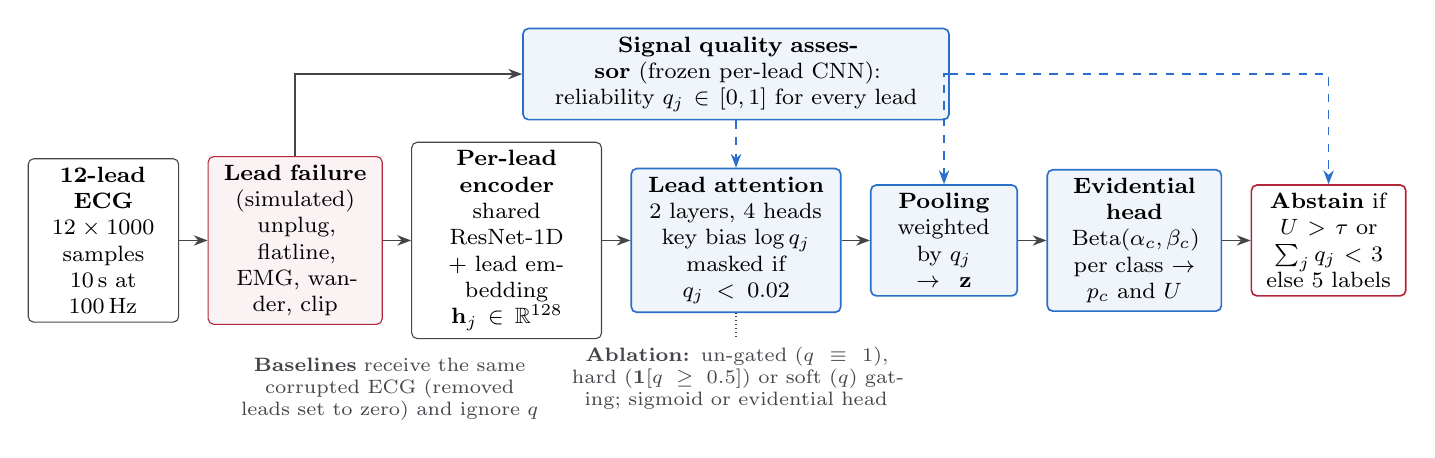
\begin{tikzpicture}[
    font=\footnotesize,
    >={Stealth[length=5pt]},
    box/.style={draw=inkgray, rounded corners=2pt, align=center, inner sep=3pt, minimum height=1.25cm, fill=white},
    lg/.style={box, draw=lgblue, fill=lgblue!7, line width=0.6pt},
    fail/.style={box, draw=failred, fill=failred!6},
    note/.style={font=\scriptsize, text=inkgray, align=center},
    flow/.style={->, draw=inkgray, line width=0.6pt},
    qflow/.style={->, draw=lgblue, line width=0.6pt, dashed},
    node distance=0.36cm,
  ]
  \node[box, text width=1.7cm] (ecg) {\textbf{12-lead ECG}\\ $12\times1000$ samples\\ 10\,s at 100\,Hz};
  \node[fail, right=of ecg, text width=2.0cm] (fail) {\textbf{Lead failure}\\ (simulated)\\ unplug, flatline,\\ EMG, wander, clip};
  \node[box, right=of fail, text width=2.2cm] (enc) {\textbf{Per-lead encoder}\\ shared ResNet-1D\\ + lead embedding\\ $\mathbf{h}_j\in\mathbb{R}^{128}$};
  \node[lg, right=of enc, text width=2.45cm] (mala) {\textbf{Lead attention}\\ 2 layers, 4 heads\\ key bias $\log q_j$\\ masked if $q_j<0.02$};
  \node[lg, right=of mala, text width=1.65cm] (pool) {\textbf{Pooling}\\ weighted by $q_j$\\ $\rightarrow\ \mathbf{z}$};
  \node[lg, right=of pool, text width=2.0cm] (head) {\textbf{Evidential head}\\ Beta$(\alpha_c,\beta_c)$\\ per class $\rightarrow$\\ $p_c$ and $U$};
  \node[box, right=of head, text width=1.75cm, draw=failred, line width=0.6pt] (abst) {\textbf{Abstain} if\\ $U>\tau$ or $\sum_j q_j<3$\\ else 5 labels};

  \node[lg, above=0.6cm of mala, text width=5.2cm, minimum height=0.75cm] (sqa)
       {\textbf{Signal quality assessor} (frozen per-lead CNN):\\ reliability $q_j\in[0,1]$ for every lead};

  \draw[flow] (ecg) -- (fail);
  \draw[flow] (fail) -- (enc);
  \draw[flow] (enc) -- (mala);
  \draw[flow] (mala) -- (pool);
  \draw[flow] (pool) -- (head);
  \draw[flow] (head) -- (abst);
  \draw[flow] (fail.north) |- (sqa.west);
  \draw[qflow] (sqa.south) -- (mala.north);
  \draw[qflow] (sqa.east) -| (pool.north);
  \draw[qflow] (sqa.east) -| (abst.north);

  \node[note, below=0.3cm of mala, text width=5.4cm] (abl)
       {\textbf{Ablation:} un-gated ($q\equiv1$), hard ($\mathbf{1}[q\ge0.5]$) or soft ($q$) gating;
        sigmoid or evidential head};
  \draw[densely dotted, draw=inkgray] (abl.north) -- (mala.south);
  \node[note, below=0.3cm of fail, text width=4.2cm, xshift=1.2cm]
       {\textbf{Baselines} receive the same corrupted ECG (removed leads set to zero) and ignore $q$};
\end{tikzpicture}
\caption{The evaluated pipeline. Lead failure is simulated in training and at test time. A frozen quality assessor
scores every lead; its score $q_j$ biases the lead-attention keys, weights the pooling and enters one of the two
abstention rules. The ablations (bottom) remove the gating or replace the evidential head with a sigmoid head. The
baselines receive the same corrupted ECG, with removed leads set to zero.}
\label{fig:overview}
\end{figure*}


\IEEEPARstart{T}{he} standard electrocardiogram (ECG) records ten seconds from ten electrodes and derives twelve
leads, and its interpretation assumes that each electrode sits where the recording conventions place it
\cite{kligfield2007recommendations}. In emergency departments, ambulances and intensive-care units this assumption
does not always hold. Electrodes lose contact, cables are pulled during transfers, muscle activity adds noise, and
cables can be connected to the wrong electrodes, which can imitate disease \cite{batchvarov2007incorrect}. An
automated classifier used in these settings therefore receives recordings that differ from those it was trained
on.

Deep networks trained on large collections of 12-lead ECGs classify common abnormalities with high accuracy
\cite{ribeiro2020automatic}; on PTB-XL the reference benchmark reports a macro-averaged area under the receiver
operating characteristic curve (macro-AUROC) of about 0.93 for five diagnostic superclasses
\cite{strodthoff2021benchmark}. A convolutional network has no explicit representation of a missing or corrupted
channel, so it returns a diagnosis whatever the state of the input. Three kinds of remedy have been used. The
training data can include recordings with leads removed, as in random lead masking \cite{oh2022leadagnostic},
modality dropout in multimodal learning \cite{neverova2016moddrop}, and the reduced-lead models of the
PhysioNet/Computing in Cardiology Challenge 2021 \cite{reyna2021willtwodo,nejedly2022ensemble}. Information about
signal quality, long studied for ECG acceptability and alarm reduction \cite{clifford2012sqi,behar2013sqi}, can be
passed to the model so that it relies less on poor leads. And the model can estimate its own uncertainty, for
example with evidential deep learning \cite{sensoy2018edl}, so that the system can abstain.

These remedies are often combined. If a quality-aware or uncertainty-aware model is trained on corrupted recordings
and compared with a baseline trained on clean ones, any difference mixes the effect of the architecture with that
of the training data. We therefore ask a narrower question: once a classifier is trained with simulated lead
failure, does gating its lead attention by a per-lead quality estimate, or adding an evidential output that can
abstain, improve robustness or make its uncertainty more useful?

We built a pipeline that contains both components (Fig.~\ref{fig:overview}). A frozen signal-quality assessor
scores every lead, a lead-attention network uses the scores to down-weight or exclude unreliable leads, and a
per-class Beta-evidential output reports an uncertainty that drives abstention. We trained this model, three
ablations that remove the gating or replace the evidential output, and five baselines under one training budget,
and tested all of them on the same deterministically corrupted copies of the PTB-XL test fold, with an oracle
quality control and paired bootstrap intervals. The gated and evidential models were trained only with
corruption, so the study measures what these components add to corruption training, not what they would achieve
without it.

The contributions are three empirical results on PTB-XL with simulated lead failure:
\begin{itemize}
  \item Training with simulated lead failure accounts for most of the difference between models under lead loss:
        the same residual network (ResNet) gains \gainDropKTen{} macro-AUROC with ten of twelve leads removed and
        loses nothing on complete recordings (Section~\ref{sec:res-dropout}).
  \item With that training, hard and soft quality gating show no measurable advantage over un-gated lead
        attention, and the full system is not significantly better than a corruption-trained ResNet in any of
        \bootNRows{} paired comparisons; it is worse under baseline wander and strong muscle noise
        (Section~\ref{sec:res-gating}).
  \item The evidential uncertainty ranks errors no better than the model's predicted probabilities and does not
        increase as leads are removed, while discrimination falls; abstention beyond the clean-data rate comes only
        from a rule that counts usable leads (Section~\ref{sec:res-edl}).
\end{itemize}
The code, trained models and result files are publicly available (see the first-page footnote).

\section{Related Work}
\label{sec:related}

\subsection{Classification from reduced and missing leads}
The question of how much of the twelve-lead ECG a classifier really needs was put to the community by the
PhysioNet/Computing in Cardiology Challenge 2021, \emph{Will Two Do?}, which asked whether reduced-lead
recordings retain the diagnostic information of the full twelve leads \cite{reyna2021willtwodo}. The winning
entry, an ensemble of residual convolutional networks with a multi-head attention mechanism, ranked first in every
lead configuration, with nearly unchanged scores from twelve down to two leads on the hidden validation set
\cite{nejedly2021cinc,nejedly2022ensemble}. In representation learning, Oh \emph{et al.}\ pre-train ECG encoders with random lead
masking so that the learned features do not depend on a fixed set of leads \cite{oh2022leadagnostic}.

These works share a premise: the model is told, or trained to expect, that some leads are absent. Our setting
differs in two ways. First, failure is unannounced: the input is always a twelve-lead array, and a failed lead
arrives as zeros, a flat line or noise. Second, our aim is not a better reduced-lead classifier but a controlled
attribution: given that training already includes lead failure, as in lead masking, does an explicit per-lead
quality estimate that gates the attention add anything? Our answer, that the augmentation carries almost all of
the benefit, is consistent with the success of masking-based training in this prior work.

\subsection{Benchmarks on PTB-XL}
Strodthoff \emph{et al.}\ established the reference benchmark for PTB-XL with its recommended patient-level folds;
convolutional networks, in particular ResNet- and Inception-based architectures, performed best across tasks
\cite{strodthoff2021benchmark}. We adopt the same folds, label definition and 100\,Hz signal. Our models are
trained under a deliberately small, shared budget and do not reach the benchmark's absolute scores
(Section~\ref{sec:res-clean}); every comparison in this paper is therefore relative, between models trained
identically.

\subsection{Evidential deep learning and its critics}
Evidential deep learning places a Dirichlet distribution over class probabilities, interprets the network
outputs as evidence in the sense of subjective logic, and reads uncertainty from the total amount of evidence,
all from a single deterministic network \cite{sensoy2018edl}. Its original evaluation reported strong
out-of-distribution detection and robustness to adversarial perturbation. Its theoretical footing has since been
questioned. Bengs \emph{et al.}\ showed that the loss functions used to train such second-order predictors do not
incentivise them to represent their epistemic uncertainty faithfully \cite{bengs2022pitfalls}. Shen
\emph{et al.}\ sharpened this analysis across many evidential objectives, found that the learned epistemic
uncertainty does not vanish even with infinite data, and argued that evidential models behave more like
energy-based out-of-distribution detectors, which can still perform well on downstream tasks despite poor
uncertainty quantification \cite{shen2024mirage}.

Our results add a concrete, applied data point to this debate. Lead failure is a structured loss of information
whose severity we control exactly, and the evidential uncertainty of our model does not track it
(Section~\ref{sec:res-edl}). Unlike in an out-of-distribution benchmark, a recording with failed leads
contains strictly less information than the same recording intact, so an uncertainty measure that stays flat
as leads disappear is hard to defend.

\subsection{Calibration and selective prediction}
Modern networks are often poorly calibrated, and a single temperature fitted on held-out data is a simple and
effective remedy \cite{guo2017calibration}; we apply it to every sigmoid model so that calibration comparisons
with the evidential head are fair. Selective classification lets a classifier abstain to reach a target risk;
thresholding the network's own maximum class probability is already a strong rejection rule
\cite{geifman2017selective}. Our confidence score is the multi-label analogue of that rule, and our
risk--coverage results show that it matches the evidential uncertainty (Section~\ref{sec:res-edl}).

\subsection{What this study adds}
We do not propose a new architecture. We contribute a controlled ablation that separates three ingredients that
are usually introduced together (training with lead failure, quality-gated lead attention and evidential
abstention), evaluates them on identical, deterministically corrupted test data, controls for the accuracy of
the quality estimate with an oracle, and reports paired confidence intervals. The value of the study lies in
which of these ingredients survive that separation.

\section{Data and Simulated Lead Failure}
\label{sec:data}

\subsection{PTB-XL}
\label{sec:data-ptbxl}
We use PTB-XL version~1.0.3 \citeneeded{PTB-XL dataset paper (Wagner et al.) and PhysioNet v1.0.3 record, DOI
10.13026/kfzx-aw45}, a public collection of clinical 12-lead ECGs of 10\,s each, annotated with SCP-ECG
statements. We use the 100\,Hz release, so every record is a $12\times1000$ array in the fixed lead order I, II,
III, aVR, aVL, aVF, V1--V6. Labels are the five diagnostic superclasses: normal ECG (NORM), myocardial infarction
(MI), ST/T change (STTC), conduction disturbance (CD) and hypertrophy (HYP). Every statement marked as diagnostic
is mapped to its superclass irrespective of its likelihood value, records may carry several superclasses
(multi-label), and records without any diagnostic superclass are excluded, leaving \nRecordsKept{} records. We follow the dataset's recommended stratified folds \citeneeded{PTB-XL paper
on \texttt{strat\_fold}}: folds 1--8 for training, fold~9 for validation and fold~10 (\nTestRecords{} records) for
testing. Each lead of each record is standardised to zero mean and unit variance; a lead whose standard deviation
is below $10^{-6}$ (a dead lead) is set to zero instead of being divided by a near-zero number. The raw
millivolt signal is kept only for display.

\subsection{A severity model of lead failure}
\label{sec:data-failure}
Every corruption acts on a batch $\mathbf{x}\in\mathbb{R}^{B\times12\times T}$ and returns the corrupted signal
together with a per-lead \emph{severity} $s_j\in[0,1]$, where $s_j=0$ means the lead is untouched (exactly) and
$s_j=1$ means it carries no usable signal. Severity defines the ground truth for the quality assessor,
$q^\ast_j=1-s_j$, and the binary label ``reliable'' $\Leftrightarrow s_j<0.5$. Five failure types are simulated
(Fig.~\ref{fig:corruptions}):
\begin{itemize}\setlength{\itemsep}{1pt}
  \item \emph{Removal}: the lead is set to zero ($s_j=1$), as when an electrode detaches.
  \item \emph{Flatline}: the lead holds its first sample, as with a stuck amplifier ($s_j=1$).
  \item \emph{Muscle (EMG) noise}: white noise band-limited to 20--45\,Hz in the Fourier domain and scaled to a
        target signal-to-noise ratio relative to the lead's own power; $s_j=1-\mathrm{clip}(\mathrm{SNR}_{\mathrm{dB}}/20,0,1)$.
        Mains interference (50/60\,Hz) is deliberately not simulated: it lies at or above the Nyquist frequency of
        the 100\,Hz signal and cannot be represented.
  \item \emph{Baseline wander}: a sinusoid of 0.1--0.5\,Hz with an amplitude of 0.5--3 times the lead's standard
        deviation, as from respiration or movement; $s_j=\mathrm{clip}(r/2,0,1)$ for amplitude ratio $r$.
  \item \emph{Amplitude clipping}: saturation at a percentile (70--95) of $|x|$; $s_j$ is the clipped fraction
        divided by 0.2, capped at~1.
\end{itemize}

\begin{figure*}[t]
\centering
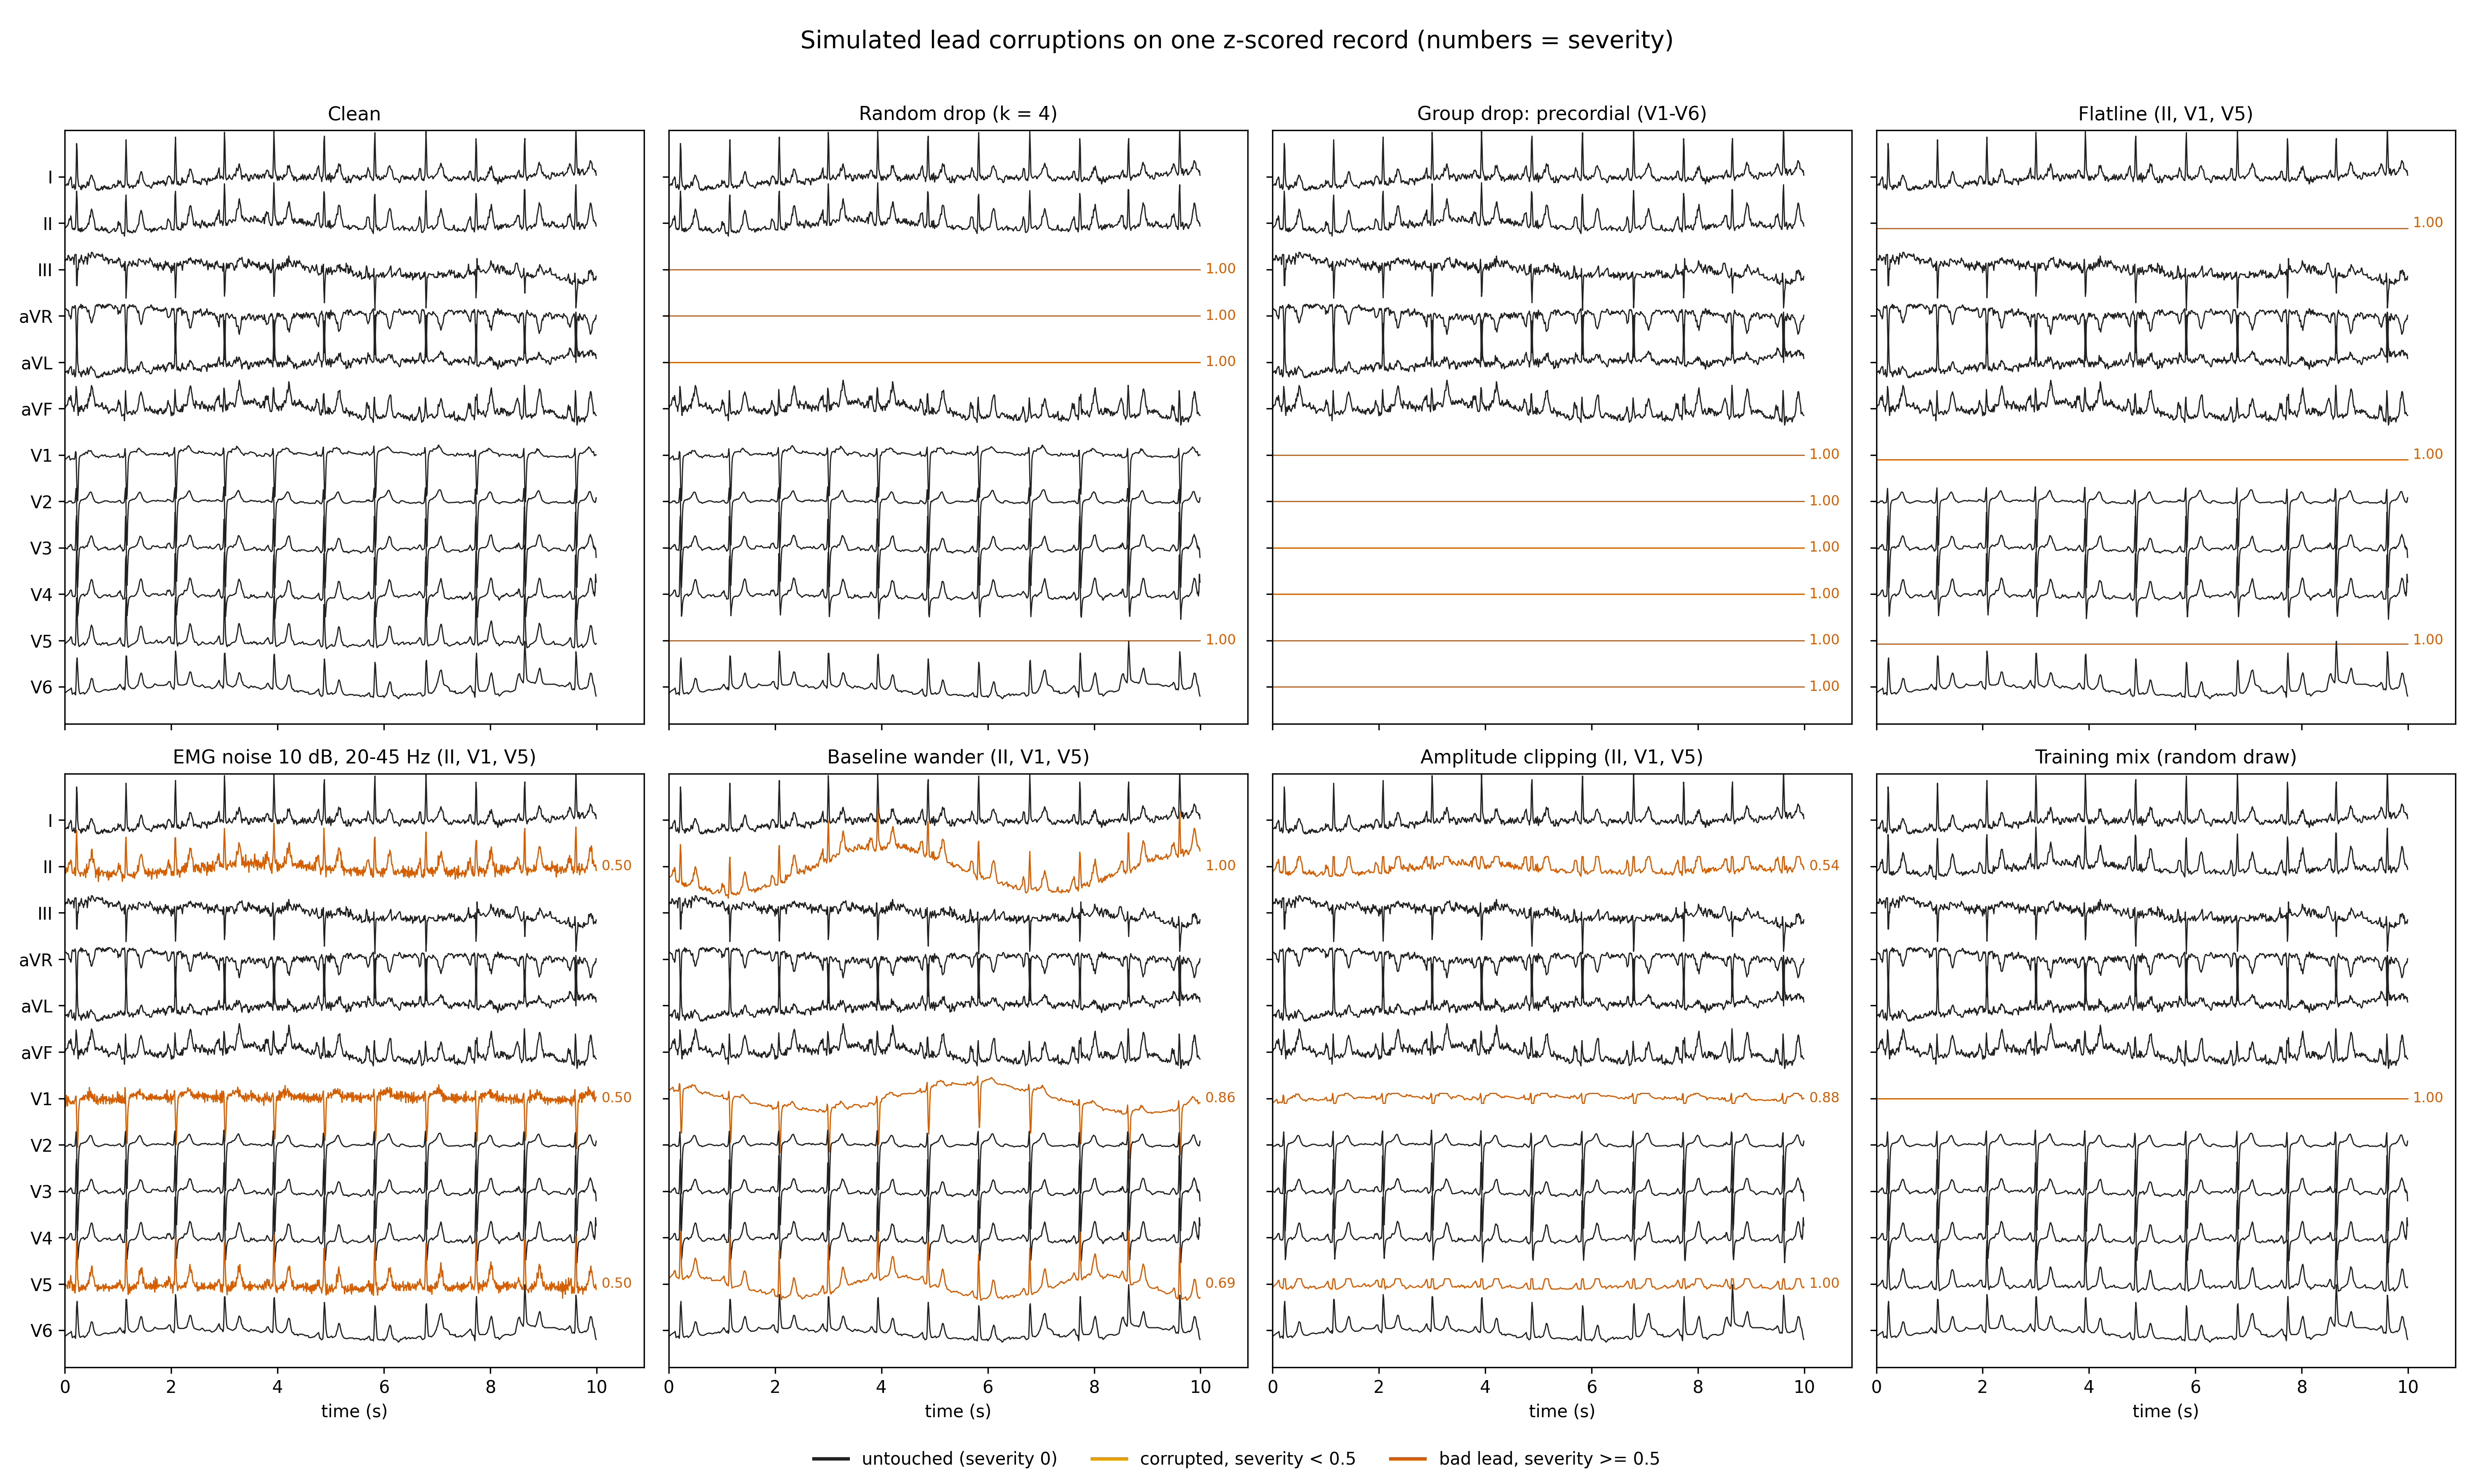
\includegraphics[width=0.92\textwidth]{corruption_examples.png}
\caption{The simulated failure types applied to one PTB-XL record (z-scored). Numbers give each lead's severity
$s_j$; black leads are untouched ($s_j=0$), light-orange leads are corrupted but still counted as reliable
($s_j<0.5$), dark-orange leads are unreliable ($s_j\ge0.5$). The last panel is one random draw of the training
mixture.}
\label{fig:corruptions}
\end{figure*}

\subsection{Training-time corruption}
\label{sec:data-train}
During training, corruption is sampled independently for every record of every batch. With probability 0.30 an
artifact (EMG noise with an SNR drawn uniformly from 0--20\,dB, baseline wander or clipping) is applied to one to
three random leads; with probability 0.50, zero to six random leads are removed, a quarter of them by flatlining
instead of zeroing; with probability 0.15, an entire lead group is removed (all precordial leads, all limb leads,
or V1--V3). These events can combine, artifacts are applied before removals, and the severity of a lead hit
twice is the larger of the two. If fewer than two reliable leads would remain, the least-corrupted leads are
restored, so every training record keeps at least two.

\subsection{Test-time conditions}
\label{sec:data-test}
For evaluation, the whole test fold is corrupted once per condition, on the CPU, with a random generator seeded
by the condition's name and draw, so that every model sees bit-identical inputs. The conditions are: the clean test
fold; random removal of $k\in\{0,2,4,6,8,10\}$ leads, three independent draws each; removal of the precordial
leads (V1--V6), the limb leads (I, II, III, aVR, aVL, aVF) or V1--V3; and EMG noise at 10\,dB, baseline wander or
clipping on two, four or six random leads. That makes 31 conditions including the clean one. EMG at 10\,dB has a
severity of exactly 0.5, on the boundary of the reliable label; we keep it because it is the realistic
operating point, and report the quality assessor's agreement both with and without such ambiguous leads
(Section~\ref{sec:setup}).

\section{Models}
\label{sec:method}

All neural models map a (possibly corrupted) record $\mathbf{x}\in\mathbb{R}^{12\times1000}$ to five class
probabilities. The quality-aware models additionally receive a per-lead reliability vector
$\mathbf{q}\in[0,1]^{12}$; every other model ignores it and sees removed leads as zeros. Table~\ref{tab:models}
summarises the nine variants.

\begin{table}[t]
\centering
\caption{The evaluated models. ``Missing leads'' states how a failed lead reaches the model. Seeds: number of
independent training runs.}
\label{tab:models}
\begin{adjustbox}{max width=\columnwidth}
\begin{tabular}{@{}llccc@{}}
\toprule
Model & Missing leads & Corrupt.\ training & Params & Seeds \\
\midrule
XGBoost (per-lead statistics) & NaN features & -- & -- & 1 \\
MLP & zero-filled & yes & \paramsMlp & 1 \\
ResNet-1D, clean-trained & zero-filled & no & \paramsRes & 1 \\
ResNet-1D, corruption-trained & zero-filled & yes & \paramsRes & 3 \\
Patch Transformer & zero-filled & yes & \paramsTrans & 1 \\
ResNet + lead attention (un-gated) & zero-filled & yes & \paramsResAttn & 1 \\
LG-hard (binary mask) & $\mathbf{1}[q\ge0.5]$ & yes & \paramsLgHard & 1 \\
LG-soft (soft gating) & $q$ & yes & \paramsLgSoft & 1 \\
LG-EDL (soft gating + evidential head) & $q$ + abstention & yes & \paramsLgEdl & 3 \\
\bottomrule
\end{tabular}
\end{adjustbox}
\end{table}

\subsection{Signal quality assessor}
\label{sec:method-sqa}
The assessor is a small convolutional network applied to each lead independently and shared across leads
(\paramsSqa{} parameters): four blocks of a 1-D convolution (kernel 7, stride 2; 16, 32, 64 and 64 channels),
batch normalisation and GELU, followed by concatenated global average and max pooling, a linear layer and a
sigmoid, giving one score $q_j\in[0,1]$ per lead. It is trained on the training folds with the training-time
corruption of Section~\ref{sec:data-train}, drawn afresh for every batch, using binary cross-entropy against the
soft target $q^\ast_j=1-s_j$, for \sqaEpochs{} epochs with AdamW (learning rate $10^{-3}$, weight decay
$10^{-2}$), cosine decay and batches of 128; the epoch with the lowest validation loss is kept. It is then
frozen. During classifier training and at test time it scores
the \emph{corrupted} signal, exactly as it would in deployment; no classifier ever sees the true severities.

\subsection{Per-lead encoder}
\label{sec:method-encoder}
Each lead is encoded on its own by one shared ResNet-1D: a stem convolution (kernel 7, stride 2, 32 channels),
three residual stages of 32, 64 and 128 channels (each with two kernel-7 convolutions, stride 2, batch
normalisation and GELU), global average pooling and a linear projection to $d=128$. A learned embedding of each
lead's position is added, giving tokens $\mathbf{h}_j\in\mathbb{R}^{128}$, $j=1,\dots,12$ (\paramsLgEncoder{}
parameters). Because the encoder never mixes leads, a lead's token depends on that lead alone.

\subsection{Mask-aware lead attention}
\label{sec:method-mala}
The twelve tokens pass through two pre-norm transformer layers with four heads, a feed-forward width of 256 and
dropout 0.1 on the feed-forward and residual branches (never on the attention weights), \paramsLgAttention{}
parameters in total. Attention is written out explicitly so that lead quality can enter as an additive bias on
the keys:
\begin{equation}
\mathbf{A}=\operatorname{softmax}\!\left(\frac{\mathbf{Q}\mathbf{K}^{\top}}{\sqrt{d_k}}+\mathbf{1}\mathbf{b}^{\top}\right),
\label{eq:attn}
\end{equation}
\begin{equation}
b_j=\begin{cases}\log\max(q_j,10^{-6}) & \text{if } q_j\ge0.02,\\ -10^{9} & \text{if } q_j<0.02,\end{cases}
\label{eq:bias}
\end{equation}
with the softmax over keys $j$ and $d_k=32$. A lead of reliability $q_j$ thus has its attention weight scaled by
$q_j$ before renormalisation, and a lead below the floor of 0.02 is excluded. After the last layer, the output
tokens $\mathbf{h}'_j$ are pooled with the same weights,
\begin{equation}
\mathbf{z}=\frac{\sum_j w_j\,\mathbf{h}'_j}{\sum_j w_j+10^{-6}},\qquad w_j=q_j\,\mathbf{1}[q_j\ge0.02].
\label{eq:pool}
\end{equation}
If every lead of a record falls below the floor, the lead with the highest $q_j$ is kept with bias 0 and weight 1,
so the output is always defined.

\emph{Exact invariance.} If lead $j$ is below the floor and at least one lead is not, the output does not depend
on $\mathbf{x}_j$ at all: its token enters no other token's update because its attention weight is exactly zero
in floating point ($e^{-10^{9}}$ underflows to 0), its own output token is pooled with weight zero, and the
encoder, layer normalisation and evaluation-mode batch normalisation never mix leads. The released tests check
this to within $10^{-5}$ by replacing such leads with large random noise.

The three gating variants share this code and differ only in $\mathbf{q}$: \emph{soft} gating uses the
assessor's score, \emph{hard} gating uses $\mathbf{1}[q_j\ge0.5]$ (ties in the all-floored case broken by the soft
score), and the \emph{un-gated} control sets $q_j\equiv1$, which reduces Eqs.~\eqref{eq:attn}--\eqref{eq:pool} to
ordinary self-attention with mean pooling.

\subsection{Output heads}
\label{sec:method-heads}
The sigmoid head is a linear layer from $\mathbf{z}$ to five logits, trained with binary cross-entropy.

The \emph{Beta-evidential head} maps $\mathbf{z}$ to ten non-negative evidence values through a linear layer and
a softplus, $e^{+}_k$ and $e^{-}_k$ for each class $k$, and sets $\alpha_k=e^{+}_k+1$, $\beta_k=e^{-}_k+1$. The
class is then described by a Beta distribution over its probability, with
\begin{equation}
p_k=\frac{\alpha_k}{\alpha_k+\beta_k},\qquad u_k=\frac{2}{\alpha_k+\beta_k},\qquad U=\frac{1}{5}\sum_{k=1}^{5}u_k .
\label{eq:edl}
\end{equation}
With no evidence ($\alpha_k=\beta_k=1$) the uncertainty $u_k$ is 1; it shrinks as evidence accumulates. Training
minimises, per class, the expected binary cross-entropy under the Beta distribution plus a regulariser that
removes misleading evidence,
\begin{align}
\mathcal{L}_k={}&y_k\big[\psi(\alpha_k+\beta_k)-\psi(\alpha_k)\big]\nonumber\\
&+(1-y_k)\big[\psi(\alpha_k+\beta_k)-\psi(\beta_k)\big]\nonumber\\
&+\lambda_t\,\mathrm{KL}\!\left(\mathrm{Beta}(\tilde\alpha_k,\tilde\beta_k)\,\|\,\mathrm{Beta}(1,1)\right),
\label{eq:edlloss}
\end{align}
where $\psi$ is the digamma function, $(\tilde\alpha_k,\tilde\beta_k)=(1,\beta_k)$ if $y_k=1$ and
$(\alpha_k,1)$ if $y_k=0$, and $\lambda_t=\min(1,t/10)$ for epoch $t=0,1,\dots$ The loss is summed over classes
and averaged over the batch. This is the cross-entropy variant (Eq.~4) of evidential deep learning
\cite{sensoy2018edl}, applied per class with a two-outcome Dirichlet, i.e.\ a Beta distribution, so
that it suits multi-label diagnosis; the original work used a squared-error variant in its own experiments. We
verified the closed-form terms of Eq.~\eqref{eq:edlloss} against numerical integration (agreement to
$2\times10^{-11}$).

\subsection{Abstention}
\label{sec:method-abstain}
LG-EDL abstains on a whole record when either
\begin{equation}
U>\tau\qquad\text{or}\qquad\textstyle\sum_{j=1}^{12}q_j<3,
\label{eq:abstain}
\end{equation}
that is, when the evidential head reports high uncertainty or when less than about three leads' worth of usable
signal remains. The threshold $\tau$ is the 95th percentile of $U$ on the clean validation fold, so the first
rule rejects 5\% of clean validation records by construction.

\subsection{Baselines}
\label{sec:method-baselines}
\emph{XGBoost} receives eight statistics per lead (mean, standard deviation, minimum, maximum, skewness,
kurtosis, dominant frequency and peak-to-peak amplitude; 96 features). A flat lead (standard deviation below
$10^{-6}$) has all its features set to missing, which gradient-boosted trees handle natively. One binary
classifier per class is trained (at most 500 trees of depth 4, learning rate 0.05, row and column subsampling 0.8,
early stopping after 30 rounds without improvement in validation AUROC). The \emph{MLP} flattens the record into
12\,000 inputs, followed by layers of 512 and 128 units with GELU and dropout 0.3. The \emph{ResNet-1D} treats the
twelve leads as input channels: a stem convolution to 64 channels and four residual stages of 64, 64, 128 and 128
channels (stride 2 each), global average pooling and a linear layer to 128. The \emph{patch Transformer} cuts the
record into 40 patches of 25 samples across all twelve leads, embeds them, adds learned positions and applies the
same two-layer, four-head, $d=128$ encoder as the lead attention, followed by mean pooling. The un-gated
\emph{ResNet + lead attention} is the lead-attention model with $q_j\equiv1$ (Section~\ref{sec:method-mala}), so
it differs from LG-soft only in the gating.

\section{Experimental Setup}
\label{sec:setup}

\subsection{Training}
\label{sec:setup-train}
All neural models share one training recipe and budget, with no per-model tuning: AdamW (learning rate
$10^{-3}$, weight decay $10^{-2}$), cosine learning-rate decay over all steps, batches of 128, at most 15 epochs,
and early stopping with a patience of four epochs on the macro-AUROC of the clean validation fold, whose best
checkpoint is the one evaluated. Mixed precision is used on the GPU. Corruption-trained models corrupt every batch
on the fly (Section~\ref{sec:data-train}); the quality-aware models receive $\mathbf{q}$ from the frozen assessor
applied to that corrupted batch. LG-EDL uses Eq.~\eqref{eq:edlloss}, all other neural models binary
cross-entropy. LG-EDL and the corruption-trained ResNet, the two models the main comparison rests on, were trained
with three seeds (0, 1, 2); every other variant with one. The full run list (twelve neural trainings and
XGBoost) took \gpuMinutes{} minutes of wall-clock time in total on a single GPU machine.

\subsection{Post-hoc fitting on the validation fold}
\label{sec:setup-fit}
Three quantities are fitted on clean validation predictions only, never on test data. (i) Every model except
LG-EDL receives one temperature $T$, applied as $\sigma(\mathrm{logit}(p)/T)$ and chosen to minimise the binary
cross-entropy over all five classes ($T\in[e^{-3},e^{3}]$), so that calibration comparisons with the evidential
head are fair. (ii) Each model receives a decision threshold per class that maximises that class's F1 score
(grid 0.01--0.99). (iii) LG-EDL receives the abstention threshold $\tau$ of Section~\ref{sec:method-abstain}.

\subsection{Metrics}
\label{sec:setup-metrics}
The primary metric is the macro-averaged area under the ROC curve over the five classes (macro-AUROC), which does
not depend on thresholds. We also report macro-F1 at the tuned thresholds, per-class AUROC, and the expected
calibration error (ECE) computed over all $N\times5$ binary predictions in 15 equal-width bins.

\emph{Selective prediction.} For multi-label outputs we define the per-record risk as the fraction of the five
labels predicted wrongly at the tuned thresholds. Records are sorted by an uncertainty score, from most to least
certain, and the risk among the kept records is reported at 20 coverage levels from 5\% to 100\%. LG-EDL is
scored with its evidential uncertainty $U$ and, for a like-for-like comparison, with the confidence score
$1-\frac{1}{5}\sum_k\max(p_k,1-p_k)$ that is used for every other model.

\emph{Statistical comparison.} The main comparison, LG-EDL against the corruption-trained ResNet, uses a paired
bootstrap over test records: in each of \bootNBoot{} resamples, both models' macro-AUROC are computed on the same
records, each averaged over its three seeds, and the 95\% interval of the difference is taken from the
percentiles. Intervals are reported per condition and are not corrected for multiple comparisons; we discuss
this where it matters (Section~\ref{sec:res-gating}).

\emph{Oracle control.} To separate the value of gating from the accuracy of the quality estimate, the gated
models are also evaluated with the true reliability $q^\ast_j=1-s_j$ in place of the assessor's estimate.

\emph{Quality-assessor check.} The assessor's lead-level agreement, the accuracy of $\mathbf{1}[q_j\ge0.5]$ against
the reliable label $\mathbf{1}[s_j<0.5]$, is measured on corrupted copies of the test fold, both over all leads
and excluding the ambiguous band $|s_j-0.5|<0.1$. Excluding that band, the lowest agreement over all failure
types is \sqaGate{} (\sqaGateType); including it, EMG at the test SNR, whose severity sits exactly on the
boundary, is matched on only \sqaEmgTestCorrupted{} of its corrupted leads.

\subsection{Reproducibility}
\label{sec:setup-repro}
Every training run is resumable from atomic checkpoints that store all random-number states, and the test-time
corruption is deterministic. Twenty unit tests, including exact invariance of the masked models to replaced
leads, attention rows that sum to one with zeros on masked keys, deterministic test corruption and an overfitting
check, pass before any training. All tables and numbers in this paper are generated by a script directly from the
released result files.

\section{Results}
\label{sec:results}

All results are on the PTB-XL test fold (fold~10, \nTestRecords{} records), and all models receive the same corrupted
test data for each condition. Values for LG-EDL and the corruption-trained ResNet are mean\,$\pm$\,standard deviation
over three seeds; the other variants were trained once. For random lead removal, each value is first averaged over
the three draws of that condition.

% ---------------------------------------------------------------------------------------------------------------
\subsection{Clean Test Performance}
\label{sec:res-clean}

\begin{table}[t]
\centering
\caption{Clean test performance. Mean\,$\pm$\,standard deviation over three seeds where available, otherwise one
run. ECE: expected calibration error over all $N\times5$ binary predictions (15 bins). All models except LG-EDL are
temperature-scaled on the validation fold.}
\label{tab:clean}
\begin{adjustbox}{max width=\columnwidth}% generated by make_numbers.py from results/table1.csv
\begin{tabular}{@{}lcccc@{}}
\toprule
Model & Seeds & Macro-AUROC & Macro-F1 & ECE \\
\midrule
LG-EDL & 3 & 0.903\,$\pm$\,0.001 & 0.715\,$\pm$\,0.004 & 0.032\,$\pm$\,0.011 \\
LG-soft & 1 & 0.906 & 0.715 & 0.014 \\
LG-hard & 1 & 0.907 & 0.726 & 0.012 \\
ResNet + lead attention & 1 & 0.909 & 0.726 & 0.014 \\
ResNet, corruption-trained & 3 & 0.903\,$\pm$\,0.000 & 0.706\,$\pm$\,0.005 & 0.015\,$\pm$\,0.003 \\
ResNet, clean-trained & 1 & 0.896 & 0.693 & 0.011 \\
Patch Transformer & 1 & 0.885 & 0.680 & 0.015 \\
MLP & 1 & 0.722 & 0.486 & 0.054 \\
XGBoost & 1 & 0.823 & 0.598 & 0.013 \\
\bottomrule
\end{tabular}
\end{adjustbox}
\end{table}

On complete recordings the six convolutional models, the two ResNets and the four lead-attention variants, range
from \aucResCleanClean{} (ResNet, clean-trained) to \aucResAttnClean{} (un-gated lead attention, one run)
(Table~\ref{tab:clean}). LG-EDL reaches \aucLgEdlCleanPM{} and the corruption-trained ResNet \aucResDropCleanPM; their
paired difference is \bootCleanDiff{} (95\% CI \bootCleanCI). The patch Transformer (\aucTransClean), XGBoost
(\aucXgbClean) and the MLP (\aucMlpClean) are weaker. All scores are below the published PTB-XL benchmark for the
same task at 100\,Hz, where the best single model reached \litBestSingleAuc{} and an ensemble \litEnsembleAuc{}
\cite{strodthoff2021benchmark}; with no hyperparameter tuning and at most 15 epochs, absolute performance is not
the subject of this study.

For every model, hypertrophy is the hardest class (LG-EDL \pcLgEdlHyp, corruption-trained ResNet \pcResDropHyp) and
NORM the easiest (\pcLgEdlNorm{} and \pcResDropNorm). LG-EDL has an ECE of \eceLgEdlCleanPM, against
\eceResDropCleanPM{} for the corruption-trained ResNet and between \eceResCleanClean{} and \eceResAttnClean{} for the
other ResNet and attention variants. Because only LG-EDL is not temperature-scaled, this difference does not show
that the evidential head itself is less calibrated.

% ---------------------------------------------------------------------------------------------------------------
\subsection{Training With Simulated Lead Failure}
\label{sec:res-dropout}

\begin{figure*}[t]
\centering
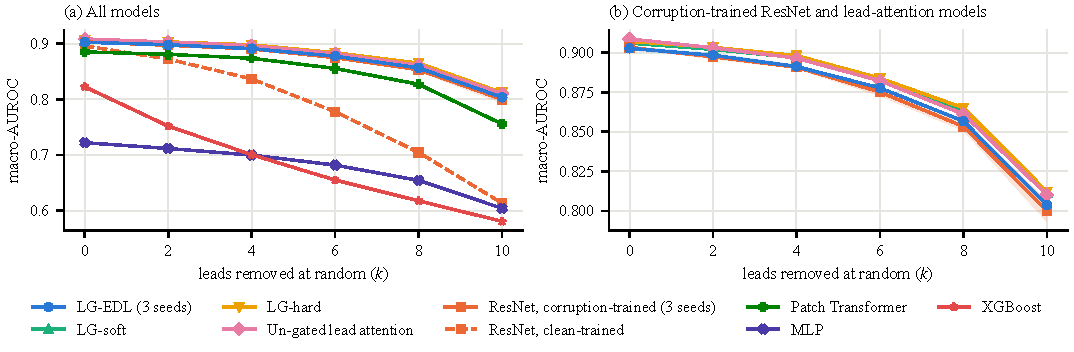
\includegraphics[width=\textwidth]{fig_random.pdf}
\caption{Macro-AUROC on the test fold as $k$ randomly chosen leads are removed (three draws per $k$). (a) All models.
(b) The five corruption-trained ResNet and lead-attention models, which overlap in (a). Bands: standard deviation
over three seeds where available.}
\label{fig:random}
\end{figure*}

\begin{table}[t]
\centering
\caption{Macro-AUROC with $k$ leads removed at random (mean over three draws, then over seeds).}
\label{tab:random}
\begin{adjustbox}{max width=\columnwidth}% generated by make_numbers.py from results/random_loss.csv (mean over 3 draws, then over seeds)
\begin{tabular}{@{}lcccccc@{}}
\toprule
& \multicolumn{6}{c}{Leads removed at random ($k$)} \\
\cmidrule(l){2-7}
Model & 0 & 2 & 4 & 6 & 8 & 10 \\
\midrule
LG-EDL & 0.903 & 0.898 & 0.891 & 0.878 & 0.857 & 0.804 \\
LG-soft & 0.906 & 0.902 & 0.897 & 0.883 & 0.863 & 0.811 \\
LG-hard & 0.907 & 0.903 & 0.898 & 0.884 & 0.865 & 0.812 \\
ResNet + lead attention & 0.909 & 0.903 & 0.897 & 0.882 & 0.861 & 0.810 \\
ResNet, corruption-trained & 0.903 & 0.897 & 0.891 & 0.875 & 0.853 & 0.800 \\
ResNet, clean-trained & 0.896 & 0.872 & 0.837 & 0.778 & 0.705 & 0.613 \\
Patch Transformer & 0.885 & 0.881 & 0.874 & 0.856 & 0.827 & 0.756 \\
MLP & 0.722 & 0.712 & 0.700 & 0.682 & 0.654 & 0.604 \\
XGBoost & 0.823 & 0.752 & 0.700 & 0.655 & 0.617 & 0.581 \\
\bottomrule
\end{tabular}
\end{adjustbox}
\end{table}

The training data separate the models more than the architecture does (Fig.~\ref{fig:random},
Table~\ref{tab:random}). The ResNet trained on clean recordings falls from \aucResCleanKZero{} with all leads to
\aucResCleanKTen{} with ten leads removed. The same architecture trained with simulated failures falls from
\aucResDropKZero{} to \aucResDropKTenPM, so at $k=10$ the two training regimes differ by \gainDropKTen. The
corruption-trained ResNet loses nothing on clean data (\aucResDropClean{} against \aucResCleanClean). The
clean-trained ResNet is a single run, but the gap at $k=10$ is more than twenty times the seed standard deviation of
the corruption-trained ResNet. The difference also holds at the decision level: at $k=10$, macro-F1 is
\foneResCleanKTen{} for the clean-trained and \foneResDropKTen{} for the corruption-trained ResNet.

With corruption training, the ResNet and the four attention variants lie close together at $k=10$: LG-EDL
\aucLgEdlKTenPM, LG-soft \aucLgSoftKTen, LG-hard \aucLgHardKTen, un-gated attention \aucResAttnKTen{} and ResNet
\aucResDropKTen. The attention variants span \ablRangeKTen, and the best is \gapAttnResKTen{} above the ResNet. The
patch Transformer, which mixes all leads within each token, degrades more (\aucTransKTen). XGBoost, trained on clean
records and given removed leads as missing features, falls from \aucXgbKZero{} to \aucXgbKTen, and the
corruption-trained MLP from \aucMlpKZero{} to \aucMlpKTen.

\begin{table}[t]
\centering
\caption{Macro-AUROC with a lead group removed, or with an artifact on six random leads (EMG at 10\,dB, baseline
wander, clipping).}
\label{tab:group}
\begin{adjustbox}{max width=\columnwidth}% generated by make_numbers.py from results/group_loss.csv and results/artifact.csv
\begin{tabular}{@{}lcccccc@{}}
\toprule
& \multicolumn{3}{c}{Lead group removed} & \multicolumn{3}{c}{Artifact on 6 leads} \\
\cmidrule(lr){2-4}\cmidrule(l){5-7}
Model & V1--V6 & Limb & V1--V3 & EMG & Wander & Clip \\
\midrule
LG-EDL & 0.871 & 0.869 & 0.882 & 0.898 & 0.891 & 0.889 \\
LG-soft & 0.877 & 0.870 & 0.887 & 0.900 & 0.895 & 0.893 \\
LG-hard & 0.878 & 0.869 & 0.888 & 0.895 & 0.894 & 0.890 \\
ResNet + lead attention & 0.876 & 0.874 & 0.888 & 0.904 & 0.903 & 0.893 \\
ResNet, corruption-trained & 0.873 & 0.868 & 0.882 & 0.903 & 0.899 & 0.894 \\
ResNet, clean-trained & 0.747 & 0.809 & 0.851 & 0.896 & 0.844 & 0.877 \\
Patch Transformer & 0.853 & 0.845 & 0.864 & 0.885 & 0.875 & 0.880 \\
MLP & 0.661 & 0.679 & 0.669 & 0.721 & 0.684 & 0.723 \\
XGBoost & 0.666 & 0.734 & 0.743 & 0.814 & 0.749 & 0.727 \\
\bottomrule
\end{tabular}
\end{adjustbox}
\end{table}

The same pattern holds when a lead group is removed (Table~\ref{tab:group}). The precordial leads V1--V6 run across
the chest from the right sternal border to the left axillary line and record the heart in the horizontal plane
\cite{kligfield2007recommendations}; they are the main view of the anterior wall and carry much of the ST-segment,
T-wave and QRS-amplitude information. Without them, the clean-trained ResNet falls to \aucResCleanPrec, against
\aucResDropPrec{} after corruption training. The loss is not limited to infarction: for the clean-trained ResNet, the
AUROC for MI falls from \pcResCleanMi{} to \pcResCleanMiPrec, that for ST/T change from \pcResCleanSttc{} to
\pcResCleanSttcPrec, and that for NORM from \pcResCleanNorm{} to \pcResCleanNormPrec, whereas the corruption-trained
ResNet keeps \pcResDropMiPrec, \pcResDropSttcPrec{} and \pcResDropNormPrec. With baseline wander on six leads, the two
training regimes reach \aucResCleanWanderSix{} and \aucResDropWanderSix.

% ---------------------------------------------------------------------------------------------------------------
\subsection{Quality Gating}
\label{sec:res-gating}

\begin{table}[t]
\centering
\caption{Lead-attention variants (all corruption-trained): macro-AUROC on clean data, with $k=6$ and $k=10$ leads
removed at random and without V1--V6, and clean ECE. Three of the four variants are single runs.}
\label{tab:ablation}
\begin{adjustbox}{max width=\columnwidth}% generated by make_numbers.py from results/table2.csv
\begin{tabular}{@{}lcccccc@{}}
\toprule
Variant & Seeds & Clean & $k{=}6$ & $k{=}10$ & V1--V6 & ECE \\
\midrule
ResNet + lead attention & 1 & 0.909 & 0.882 & 0.810 & 0.876 & 0.014 \\
LG-hard & 1 & 0.907 & 0.884 & 0.812 & 0.878 & 0.012 \\
LG-soft & 1 & 0.906 & 0.883 & 0.811 & 0.877 & 0.014 \\
LG-EDL & 3 & 0.903 $\pm$ 0.001 & 0.878 $\pm$ 0.000 & 0.804 $\pm$ 0.002 & 0.871 $\pm$ 0.002 & 0.032 $\pm$ 0.011 \\
\bottomrule
\end{tabular}
\end{adjustbox}
\end{table}

The four attention variants share the per-lead encoder and the attention code and differ only in whether attention
and pooling are weighted by the estimated quality and in the output head (Table~\ref{tab:ablation}). Their clean
macro-AUROC spans \ablRangeClean{} and their macro-AUROC at $k=10$ spans \ablRangeKTen. The un-gated variant has the
highest clean score (\aucResAttnClean) and is never the lowest of the four under random or group lead loss. Three of
the variants are single runs and were not compared statistically; for scale, the largest seed standard deviation of
LG-EDL under random lead loss is \seedStdLgEdlMaxLoss. The ablation therefore shows no benefit of gating larger than
about 0.01 in this setting and cannot exclude a smaller one.

The paired bootstrap of LG-EDL against the corruption-trained ResNet covers the clean condition, 15 random-removal
draws, three group removals and nine artifact conditions (Appendix, Table~\ref{tab:bootstrap}). None of the
\bootNRows{} intervals lies entirely above zero. The intervals of \bootNSigNeg{} conditions lie entirely below zero,
all of them artifacts: baseline wander on two, four and six leads (\bootWanderTwoDiff, \bootWanderFourDiff,
\bootWanderSixDiff) and EMG on six leads (\bootEmgSixDiff). The intervals are uncorrected and the conditions share
test records; with \bootNRows{} comparisons at the 5\% level, about one would exclude zero by chance if the two
models were equivalent. That all four are negative and three are wander conditions suggests a systematic effect,
which we treat as tentative.

A possible reason, not tested here, is that the assessor was trained to label leads with strong wander as
unreliable, following our severity rule, so the gated models down-weight such leads although their QRS complexes
remain readable. Under wander on six leads, the three gated variants (\aucLgHardWanderSix, \aucLgSoftWanderSix,
\aucLgEdlWanderSix) score below both the un-gated model (\aucResAttnWanderSix) and the ResNet (\aucResDropWanderSix).

Two observations limit what the ablation can test. Replacing the estimated quality by the true quality changes
macro-AUROC by at most \oracleMaxAbsDiff{} for any gated run and condition, so the accuracy of the quality estimate
is not the limiting factor. And the simulated failures are easy to detect: removed leads are zero or constant, the
assessor scores untouched clean leads at \sqaMeanQClean{} on average, and its agreement with the reliability label is
at least \sqaGate{} for every failure type outside the borderline band. Its scores are therefore close to binary,
which is why hard and soft gating behave almost identically, and the soft weighting is barely exercised.

% ---------------------------------------------------------------------------------------------------------------
\subsection{Evidential Uncertainty and Abstention}
\label{sec:res-edl}

\begin{figure*}[t]
\centering
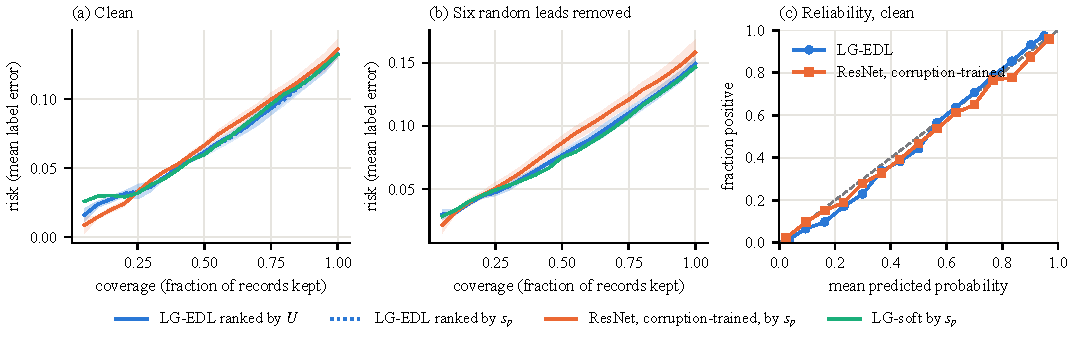
\includegraphics[width=\textwidth]{fig_riskcov.pdf}
\caption{(a, b) Risk--coverage curves: records are kept in order of increasing uncertainty, and risk is the mean
fraction of the five labels predicted wrongly at the validation-tuned thresholds; $s_p$ is the probability-based
score of Section~\ref{sec:setup-metrics}. (c) Reliability diagram on the clean test fold (LG-EDL not
temperature-scaled).}
\label{fig:riskcov}
\end{figure*}

\begin{table}[t]
\centering
\caption{Risk (mean per-record label error) at 50\%, 80\% and 100\% coverage and mean risk over 20 coverage levels
from 5\% to 100\%. $U$: evidential uncertainty; $s_p$: probability-based score.}
\label{tab:selective}
\begin{adjustbox}{max width=\columnwidth}% generated by make_numbers.py from results/risk_coverage.csv
\begin{tabular}{@{}lcccc@{}}
\toprule
Model, score & 50\% & 80\% & 100\% & Mean \\
\midrule
\multicolumn{5}{@{}l}{\emph{Clean}} \\
LG-EDL, $U$ & 0.062 & 0.102 & 0.133 & 0.068 \\
LG-EDL, confidence & 0.061 & 0.100 & 0.133 & 0.068 \\
LG-soft, confidence & 0.060 & 0.104 & 0.132 & 0.069 \\
ResNet + attn., conf. & 0.056 & 0.095 & 0.126 & 0.066 \\
ResNet (corr.), conf. & 0.066 & 0.106 & 0.136 & 0.070 \\
\midrule
\multicolumn{5}{@{}l}{\emph{6 random leads removed}} \\
LG-EDL, $U$ & 0.077 & 0.117 & 0.149 & 0.083 \\
LG-EDL, confidence & 0.077 & 0.117 & 0.149 & 0.083 \\
LG-soft, confidence & 0.075 & 0.116 & 0.147 & 0.081 \\
ResNet + attn., conf. & 0.074 & 0.115 & 0.148 & 0.082 \\
ResNet (corr.), conf. & 0.087 & 0.129 & 0.159 & 0.090 \\
\bottomrule
\end{tabular}
\end{adjustbox}
\end{table}

If the evidential head added useful uncertainty, ranking records by $U$ would give a lower risk at a given coverage
than ranking them by $s_p$ from the same model. It does not (Table~\ref{tab:selective}, Fig.~\ref{fig:riskcov}). On
clean data, LG-EDL ranked by $U$ has a risk of \riskLgEdlUCleanHalf{} at 50\% coverage, against
\riskLgEdlConfCleanHalf{} when ranked by $s_p$, and the mean risk over all coverage levels is \aurcLgEdlUClean{} for
both. With six leads removed the values are again equal (\riskLgEdlUKSixHalf{} and \riskLgEdlConfKSixHalf{} at 50\%
coverage). The lowest clean risk at 50\% coverage belongs to the un-gated attention model ranked by $s_p$
(\riskResAttnConfCleanHalf). These differences were not tested statistically.

\begin{figure*}[t]
\centering
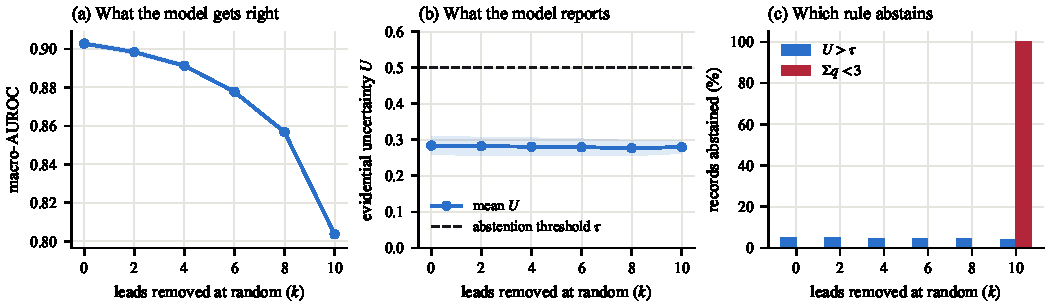
\includegraphics[width=\textwidth]{fig_certainty.pdf}
\caption{LG-EDL as leads are removed at random. (a) Macro-AUROC. (b) Mean evidential uncertainty $U$ and the
abstention threshold $\tau$. (c) Share of records rejected by each abstention rule. Lines: mean over three seeds after
averaging the three draws; bands: standard deviation over seeds.}
\label{fig:certainty}
\end{figure*}

\begin{table}[t]
\centering
\caption{LG-EDL abstention as leads are removed at random (mean over draws, then seeds). $\tau$ is the 95th
percentile of $U$ on the clean validation fold.}
\label{tab:abstain}
\begin{adjustbox}{max width=\columnwidth}% generated by make_numbers.py from results/abstain_rate.csv (LG-EDL, mean over draws then seeds)
\begin{tabular}{@{}cccccc@{}}
\toprule
$k$ & Abstain (\%) & $U{>}\tau$ (\%) & $\Sigma q{<}3$ (\%) & Mean $U$ & Mean $\Sigma q$ \\
\midrule
0 & 5.1 & 5.1 & 0.0 & 0.284 & 11.96 \\
2 & 4.8 & 4.8 & 0.0 & 0.282 & 9.97 \\
4 & 4.5 & 4.5 & 0.0 & 0.281 & 7.98 \\
6 & 4.5 & 4.5 & 0.0 & 0.279 & 5.99 \\
8 & 4.6 & 4.6 & 0.0 & 0.277 & 3.99 \\
10 & 100.0 & 4.0 & 100.0 & 0.279 & 2.00 \\
\bottomrule
\end{tabular}
\end{adjustbox}
\end{table}

$U$ also does not respond to missing leads (Fig.~\ref{fig:certainty}, Table~\ref{tab:abstain}). As $k$ goes from 0 to
10, LG-EDL's macro-AUROC falls from \aucLgEdlKZero{} to \aucLgEdlKTen, while its mean $U$ changes from \meanUKZero{}
to \meanUKTen. The $U$ rule rejects \abstainUKZero\% of test records with all leads present and between
\abstainUKTen\% and \abstainUKTwo\% for every $k$ up to ten, close to the 5\% set on validation data. The lead-count
rule never fires while four or more leads remain (mean $\sum_j q_j$ of \meanQsumKEight{} at $k=8$) and rejects every
record at $k=10$. Under lead loss, abstention beyond the clean-data rate therefore comes only from the lead-count
rule, which for these failures needs neither the evidential head nor a learned quality score.

The flat $U$ is not accompanied by a loss of calibration in LG-EDL's probabilities. Its pooled ECE is
\eceLgEdlKZero{} with all leads, \eceLgEdlKEight{} at $k=8$ and \eceLgEdlKTen{} at $k=10$, against \eceResDropKZero,
\eceResDropKEight{} and \eceResDropKTen{} for the corruption-trained ResNet. We did not record per-condition summaries
of $s_p$, so we cannot say whether the probability-based score rises with $k$.

% ---------------------------------------------------------------------------------------------------------------
\subsection{An Example Record}
\label{sec:res-case}

\begin{figure*}[t]
\centering
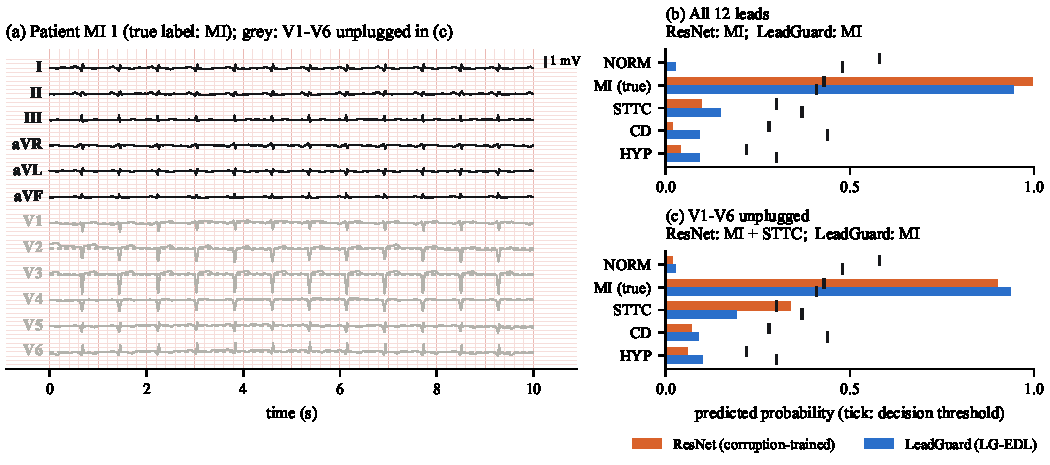
\includegraphics[width=\textwidth]{fig_vignette.pdf}
\caption{One test record before and after V1--V6 are removed. (a) The raw recording; the grey leads are removed in
(c). (b, c) Class probabilities of the corruption-trained ResNet and LG-EDL; ticks mark each model's validation-tuned
decision threshold. The record was selected from records that both models classify correctly with all leads; it
illustrates the behaviour described above and does not show how often it occurs.}
\label{fig:vignette}
\end{figure*}

Fig.~\ref{fig:vignette} shows one test record, \vigPatient, labelled MI only. With all leads both models are
correct; the ResNet gives MI a probability of \vigBaseMiFull{} and LG-EDL \vigLgMiFull. Without V1--V6, the ResNet
still detects MI (\vigBaseMiCut), but its probability for ST/T change rises from \vigBaseStFull{} to \vigBaseStCut,
above its threshold of \vigBaseStThr, so it adds a false label. LG-EDL keeps MI as its only label (\vigLgMiCut), and
its $U$ changes from \vigLgUFull{} to \vigLgUCut. On average neither pattern favours one model
(Section~\ref{sec:res-gating}).

\section{Discussion}
\label{sec:discussion}
\todo{To be drafted.}

\section{Limitations}
\label{sec:limitations}

\emph{One dataset.} All results come from PTB-XL, a single retrospective collection, used here in its 100\,Hz
version. Whether the conclusions transfer to other populations, devices, sampling rates and label sets is untested.

\emph{Simulated failures only.} Every lead failure in this study is simulated. Removed and flatlined leads are
idealised: they are exactly zero or exactly constant, and therefore trivially detectable. Real recordings fail
in subtler ways that we did not model, including intermittent electrode contact, motion artifacts with
non-stationary spectra, mains interference and swapped electrode cables \cite{batchvarov2007incorrect}, which
yields a plausible-looking but wrong signal rather than a missing one.

\emph{The quality assessor was judged against our own simulation.} Its targets are the severities of
Section~\ref{sec:data-failure}, which encode our design choices, for example that wander with an amplitude ratio
above one makes a lead unreliable. Its high agreement shows that it learned these rules, not that it would judge
real artifacts the way a clinician would. EMG at the test SNR lies exactly on the reliability boundary, where its
agreement drops to \sqaEmgTestCorrupted{} of the corrupted leads. Real, subtle artifacts may behave differently,
and soft gating, which our near-binary simulation barely exercised, might matter more there.

\emph{Limited seeds and budget.} Only the two models of the main comparison were trained with three seeds; the
ablation variants are single runs, so differences between them of the order of 0.01 macro-AUROC cannot be
ranked. No hyperparameters were tuned and training was capped at 15 epochs, which keeps the comparison fair but
leaves absolute performance below the published benchmark; stronger models might change the size, though we see
no reason for the direction, of the effects.

\emph{Statistical scope.} The paired bootstrap intervals are reported per condition, without correction for
multiple comparisons, and the conditions share test records.

\emph{One evidential variant.} We evaluated a single evidential formulation (the per-class cross-entropy variant),
trained only with corruption and without temperature scaling. Other evidential objectives, ensembles or
Monte-Carlo dropout were not compared, so the illusion of certainty is demonstrated for this model, not for
uncertainty estimation in general.

\emph{No clinical validation.} The system is a research prototype. The illustrative case and the demonstration use
hand-picked records on which both models are correct with all leads, and nothing here has been validated in a
clinical setting.

\section{Conclusion}
\label{sec:conclusion}
\todo{To be drafted.}


\appendix[Paired bootstrap by condition]
Table~\ref{tab:bootstrap} lists the paired bootstrap comparison of LG-EDL with the corruption-trained ResNet for every
test condition (Section~\ref{sec:setup-metrics}).

\begin{table}[h]
\centering
\caption{Paired bootstrap of LG-EDL minus the corruption-trained ResNet (macro-AUROC; each side averaged over three
seeds; \bootNBoot{} resamples; percentile 95\% CI). $^{*}$: CI excludes zero. Random removal is reported per draw;
$k=0$ equals the clean condition and is omitted.}
\label{tab:bootstrap}
\begin{adjustbox}{max width=\columnwidth}% generated by make_numbers.py from results/bootstrap_ci.csv (random_0 omitted: identical to clean)
\begin{tabular}{@{}lcc@{}}
\toprule
Condition & $\Delta$ macro-AUROC & 95\% CI \\
\midrule
Clean & $-$0.0006 & [$-$0.0053, +0.0039] \\
Random, $k=2$ (draw 1) & +0.0000 & [$-$0.0052, +0.0051] \\
Random, $k=2$ (draw 2) & +0.0023 & [$-$0.0027, +0.0071] \\
Random, $k=2$ (draw 3) & +0.0007 & [$-$0.0044, +0.0056] \\
Random, $k=4$ (draw 1) & $-$0.0009 & [$-$0.0062, +0.0044] \\
Random, $k=4$ (draw 2) & +0.0021 & [$-$0.0036, +0.0073] \\
Random, $k=4$ (draw 3) & $-$0.0000 & [$-$0.0058, +0.0053] \\
Random, $k=6$ (draw 1) & +0.0064 & [$-$0.0000, +0.0126] \\
Random, $k=6$ (draw 2) & $-$0.0011 & [$-$0.0071, +0.0054] \\
Random, $k=6$ (draw 3) & +0.0024 & [$-$0.0040, +0.0086] \\
Random, $k=8$ (draw 1) & +0.0036 & [$-$0.0039, +0.0109] \\
Random, $k=8$ (draw 2) & +0.0054 & [$-$0.0022, +0.0124] \\
Random, $k=8$ (draw 3) & +0.0011 & [$-$0.0054, +0.0086] \\
Random, $k=10$ (draw 1) & +0.0044 & [$-$0.0043, +0.0137] \\
Random, $k=10$ (draw 2) & +0.0006 & [$-$0.0095, +0.0097] \\
Random, $k=10$ (draw 3) & +0.0065 & [$-$0.0030, +0.0161] \\
Group: V1--V6 & $-$0.0018 & [$-$0.0070, +0.0037] \\
Group: limb & +0.0006 & [$-$0.0055, +0.0063] \\
Group: V1--V3 & +0.0003 & [$-$0.0051, +0.0056] \\
EMG 10\,dB, 2 leads & $-$0.0021 & [$-$0.0070, +0.0023] \\
EMG 10\,dB, 4 leads & $-$0.0030 & [$-$0.0079, +0.0016] \\
EMG 10\,dB, 6 leads & $-$0.0054$^{*}$ & [$-$0.0104, $-$0.0006] \\
Baseline wander, 2 leads & $-$0.0053$^{*}$ & [$-$0.0100, $-$0.0007] \\
Baseline wander, 4 leads & $-$0.0049$^{*}$ & [$-$0.0096, $-$0.0006] \\
Baseline wander, 6 leads & $-$0.0087$^{*}$ & [$-$0.0137, $-$0.0033] \\
Clipping, 2 leads & $-$0.0010 & [$-$0.0059, +0.0039] \\
Clipping, 4 leads & $-$0.0021 & [$-$0.0079, +0.0036] \\
Clipping, 6 leads & $-$0.0055 & [$-$0.0115, +0.0003] \\
\bottomrule
\end{tabular}
\end{adjustbox}
\end{table}


\section*{Acknowledgment}
This work received no specific funding, and the author declares no conflicts of interest. PTB-XL is a public,
de-identified dataset; its providers report approval of the open publication of the anonymous data by their
institutional ethics committee (\ptbxlEthicsRef) \cite{ptbxl103}.


% References: every entry in refs.bib was checked against its primary source.
\bibliographystyle{IEEEtran}
\bibliography{refs}

\end{document}
